\chapter{Validation of smearing functions}\label{cha:vali}
A full detector simulation of the \abbrATLAS detector based on the GEANT \citep{Geant4} program makes it possible to obtain the expected detector responses to electrons, muons, tau leptons, photons ($\gamma$) and jets of hadrons. However these simulations are extremely time-consuming and require a lot of computing power. Also at the present time only a limited set of these simulations exists for the \abbrATLAS phase II upgrade. In this thesis a different strategy is used. 

Instead of performing a full detector simulation of the observed particles from the event generator, which simulates the proton-proton collisions, have their energy and momenta values smeared up or down by using a probability distribution following resolution functions specific for each type of particle. The resolution functions emulate how the detector and the reconstruction are affected by the increased luminosity and the pile-up which comes with this. 

The resolution functions or smearing functions are the official functions developed from previous studies \citep{ATLAS:LOI2, ATL-PHYS-PUB-2013-004} by the \abbrATLAS collaboration for the study of the \abbrATLAS phase II upgrade. The key result of those studies was that the direction of the momenta is unaffected and that only jets and $E^{Miss}_T$ are affected by pile-up. Since this was confirmed in previous studies it was not incorporated into the smearing functions as discussed more in \sectionref{sec:smear}.

Since part of this thesis work is to take the official \abbrATLAS smearing functions and apply the smearing to each particle, it is important to check that the energy and momenta resolutions of the smeared objects are consistent with the expected values. Thus in this chapter the energy and momenta resolutions are measured after applying the smearing to some simulated processes and the resulting resolutions are compared with the expected values.

\newpage
\section{Smearing functions}\label{sec:smear}
In a simulation of a proton-proton collision all quantities such as energy, momentum and direction of all produced particles are perfectly known. In a real experiment it is only possible to get measured values from the detector. The detector energy and momentum resolutions given in the smearing functions relate the measured values to the true values on a statistical basis as:
\begin{equation}\label{eq:smear}
E' = E + \Delta E \equiv E + \sigma
\end{equation}
where $E$ is the energy at a truth level and $E'$ is the smeared energy and $\Delta E$ or $\sigma$ is a random number obtained by sampling a Gaussian distribution with mean value 0 and a standard deviation equal to the resolution for that particle, and will be denoted $\sigma$ and not cross-section as in \chapterref{cha:intro}.

The smearing functions are designed so that they take into account the efficiency of the different detectors, how they are constructed as well as their dependence on pile-up. To emulate the measured energies and momenta, the true values are smeared using the known detector resolutions given in \tableref{tab:expected sigma} which is taken from \citep{ATL-PHYS-PUB-2013-004}. 

Some terminology which is used:
\begin{itemize}
\item Energy and momenta before smearing, simulated data, is denoted at a truth level or truth data. The truth data is energy and momenta for particles directly from a Monte Carlo simulation of an event with no detector effects at all.
\item Data after smearing, which is comparable to what is measured is denoted as reconstructed data. Reconstruction is the procedure of taking electrical signals from the detectors and from these identifying particles with a specific energy and momenta. In this thesis however this is seen as equivalent to data after smearing.
\item In this thesis $p_T$ denotes the transverse momenta, $E$ the energy and $\mu$ the pile-up value.
\end{itemize}

\newpage
\begin{table}[H]
\renewcommand{\arraystretch}{1.5} %Change height of tabel
\begin{center}
\begin{tabular}{|l|l|}
\hline
Observable & Absolute $\sigma$ \\ \hline
Electron \& photon & $\sigma=0.3\oplus 0.1\sqrt{E(GeV)}\oplus 0.01E(GeV)$, $|\eta|<$ 1.4 \\
& $\sigma=0.3\oplus 0.15\sqrt{E(GeV)}\oplus 0.015E(GeV)$, 1.4 $<|\eta|<$ 2.47 \\ \hline 
Muon momentum& $\sigma=\frac{\sigma_{id} \sigma_{ms}}{\sigma_{id} \oplus \sigma_{ms}}$\\
& $\sigma_{id}=p_T(a_1 \oplus a_2 p_T)$\\
& $\sigma_{ms}=p_T(\frac{b_0}{p_T} \oplus b_1 \oplus b_2 p_T)$\\ \hline
Tau energy& $\sigma =(0.03\oplus \frac{0.76}{\sqrt{E(GeV)}})E(GeV)$, for 3 prong.\\ \hline
Jet momentum& $\sigma = p_T(GeV)(\frac{N}{p_T} \oplus \frac{S}{\sqrt{p_T}} \oplus C)$ \\ 
& where $N=a(\eta)+b(\eta)\mu$ \\ \hline
$E_T^{Miss}$ & $\sigma = (0.4+0.09\sqrt{\mu})\sqrt{\sum E(GeV)+20\mu}$ \\ \hline
\end{tabular}
\end{center}
\renewcommand{\arraystretch}{1.0} %Change back
\caption{Expected absolute $\sigma$ where the parameters are given for muons in \tableref{tab:muonparam} and for jets in \tableref{tab:jetparam}. The subscripts id and ms for the muon momentum resolution denote the parametrisation of the inner detector and the muon spectrometer. The definition of 3 prong for tau can be found in \subsectionref{sec:smear:subsec:tau}. Functions take from Ref. \citep{ATL-PHYS-PUB-2013-004}.}
\label{tab:expected sigma}
\end{table}

From the formulation of the smearing functions in \tableref{tab:expected sigma}, the biggest effect should be seen at low energies. This is related to the difficulty for the hardware triggers to select events. This means that one drawback of the high luminosity upgrade is that very low energy signal regions will be lost.

%\begin{itemize}
%\item For muon: Where a$_i$ and b$_i$ are dependent on $\eta$.
%\item For muon: All parameters are given in \tableref{tab:muonparam}.
%\item For tau: Fixed at 3 prong. 1 prong exists though was not used in this thesis. \\
%Where prong refers to the different amount of tracks that from which they were reconstructed.
%\item For Jet: Where N, S, and C depend on $\eta$. N is also dependent on the pile-up that is simulated.\\
%\item For jet: All parameters are given in %\tableref{tab:jetparam} where $N=a(\eta)+b(\eta)\mu$.
%Where $\eta$ is the same as discussed in \subsectionref{sec:eo:subsec:coord}
%\item All parameters can be found in \citep{ATL-PHYS-PUB-2013-004}.
%\end{itemize}

\begin{table}[H]
\renewcommand{\arraystretch}{1.5} %Change height of tabel
\begin{center}
\begin{tabular}{|l|l|l|l|l|l|}
\hline
 &$a_1$&$a_2$&$b_0$&$b_1$&$b_2$ \\ \hline
$\abs{\eta}\leq 1.05$&0.01607&0.000307&0.24&0.02676&0.00012 \\ \hline
$\abs{\eta}>1.05$&0.03000&0.000387&0.00&0.03880&0.00016 \\ \hline
\end{tabular}
\end{center}
\caption{Parameters used in the muon smearing function taken from Ref. \citep{ATL-PHYS-PUB-2013-004}.}
\label{tab:muonparam}
\renewcommand{\arraystretch}{1.0} %Change back
\end{table}
\begin{table}[H]
\renewcommand{\arraystretch}{1.5} %Change height of tabel
\begin{center}
\begin{tabular}{|l|l|l|l|l|}
\hline
$\abs{\eta}$&a&b&S&C \\ \hline
0-0.8&3.2&0.07&0.74&0.05 \\
0.8-1.2&3.0&0.07&0.81&0.05 \\
1.2-2.8&3.3&0.08&0.54&0.05 \\
2.8-3.6&2.8&0.11&0.83&0.05 \\ \hline
\end{tabular}
\end{center}
\caption{Parameters used in the jet smearing function taken from Ref. \citep{ATL-PHYS-PUB-2013-004}.}
\label{tab:jetparam}
\renewcommand{\arraystretch}{1.0} %Change back
\end{table}
\subsection{Electron and photon}
The identification of electrons relies on finding a hit pattern in the electromagnetic calorimeter which is consistent with that of an electron or a photon. 

If there is a track from the inner detector which can be combined with a hit then an electron has been detected. Pile-up will affect the electrons by decreasing the efficiency to identify an electron because of the increased number of tracks. However for the identified electrons the energy resolution will be close to that without pile-up. 

Photons are detected similarly to the electron though with an absence of a track and will thus be affected by pile-up similarly to the electron.

The electron and photon have the same smearing since both of their energies are measured in the electromagnetic calorimeter. 

\subsection{Muon}
The identification of muons relies on isolated tracks in the inner detector  being matched with information in the muon system. Since the muon system is the outermost detector seen from the collision point the effects of pile-up are negligible.  
\subsection{Tau}\label{sec:smear:subsec:tau}
Tau is detected similarly to the electron.
In this thesis all tau processes are for simplicity assumed to be at 3 prong, where prong refers to the number of tracks from which they were reconstructed. Such as tau decaying to 3 pions and a tau neutrino. $\tau ^{-} \rightarrow \pi ^{-} \pi ^{-} \pi ^{+} \nu _{\tau}$

This in turn means that the effect of pile-up will be worse compared to an electron as a triplet must be found in an increased number of tracks.
\subsection{Jets}\label{sec:smear:subsec:jets}
Jets as described in \subsectionref{sec:tb:subsec:jets} are cones of hadronic particles. 

The largest effect of pile-up is to add additional jets in the ATLAS detector. These additional jets contribute to additional energy deposited inside the existing jets and to $E^{Miss}_T$.
\subsection{Missing Transverse Energy}
$E_T^{Miss}$, the missing transverse energy, which was discussed in \subsectionref{sec:eo:subsec:mjet}, and defined in \eqref{eq:etmiss}, is calculated by knowing that there should be momentum conservation in the collision. It should be affected by pile-up as described in \subsectionref{sec:smear:subsec:jets}.

\newpage
\section{Validation}\label{sec:vali}
Validation is the procedure of comparing an expected resolution $\sigma$ with the resolution measured from the smeared Monte Carlo simulation. Measuring the resolution on the smeared objects uses that $E'$ and $E$ is known which through \eqref{eq:smear} can be used to statistically calculate $\sigma$. The comparison is done with Ref. \citep{ATL-PHYS-PUB-2013-004} where the resolution depending on energy, momenta and pile-up value is given in \tableref{tab:sigmaval}. The Monte Carlo simulated processes used are listed in \tableref{tab:backproc}. 

\begin{SCtable}[][ht]
\begin{tabular}{|l|l|}
\hline
Particle & Process \\ \hline
Electron & W$\rightarrow e\nu$ \\
Muon & W$\rightarrow \mu \nu$ \\
Tau & W$\rightarrow \tau \nu$ \\
$\gamma$ & $\gamma$ + jet sample \\
Jets & jet sample \\
$E_T^{Miss}$ & Z$\rightarrow \nu \nu$ + jet sample \\ \hline
\end{tabular}
\caption{Different processes from where data has been taken. Each sample is a simulation of a physical process, the simulation names can be found in \appendixref{1backpro}.}
\label{tab:backproc}
\end{SCtable}

\subsection{Method}
The energy and momentum resolutions are obtained for each type of particle by comparing the values before and after smearing.

Fitting a Gaussian curve of the smeared data from a given truth energy or momenta value will then result in the standard deviation which is used in the validation. The standard deviation is also known as the resolution of the data and will be denoted $\sigma$ and not cross-section as in \chapterref{cha:intro}.

The standard deviation is then compared to previous results \citep{ATL-PHYS-PUB-2013-004}.

The method is presented step by step below:
\begin{itemize}
\item Take a MC sample with a given particle, i.e electrons.
\item Choose electrons which have a truth energy of 75 GeV.
\item Plot the smeared electron energy for this value of truth energy. These plots are given for electrons and photons in \figureref{fig:elph}.
\item Fit a gauss function to the distribution of smeared energy and from this retrieve the sigma value of the fit.
\item Compare the measured sigma to the expected resolution given from the smearing functions.
\end{itemize}

\newpage
\section{Results}\label{cha:vali:sec:results}
As discussed above, the method was to plot the data against its smeared counterpart and through this determine $\sigma$ to see if it conforms to the expected values.

Only one energy or momenta value is shown for simplicity, though the comparison was done for different energy values. The energy is denoted $E$ and in the figures momenta is denoted $P_T$ for transverse momenta.

The average number of pile-up, explained in \subsectionref{sec:eo:subsec:pile}, is fixed at 60 as a benchmark unless anything else is stated.

As in the comparison, \figureref{fig:elph}, \figureref{fig:muon}, \figureref{fig:jet} and \figureref{fig:MET} are divided depending on the different $\eta$ values.
\newpage
\subsection{Electron and photon}\label{cha:vali:sec:res:subsec:elph}
Since these are detected very similarly in the detector, their smearing functions are identical.
The peak value represents at which value of unsmeared energy or momentum this smearing occurs. In \figureref{fig:elph} the Gaussian fit (red) and the data (black) are given for the electron energies.
%\begin{figure}[!htbp]
%  \centering 
%  \subfloat[eleta1. \label{fig:elph:1}]{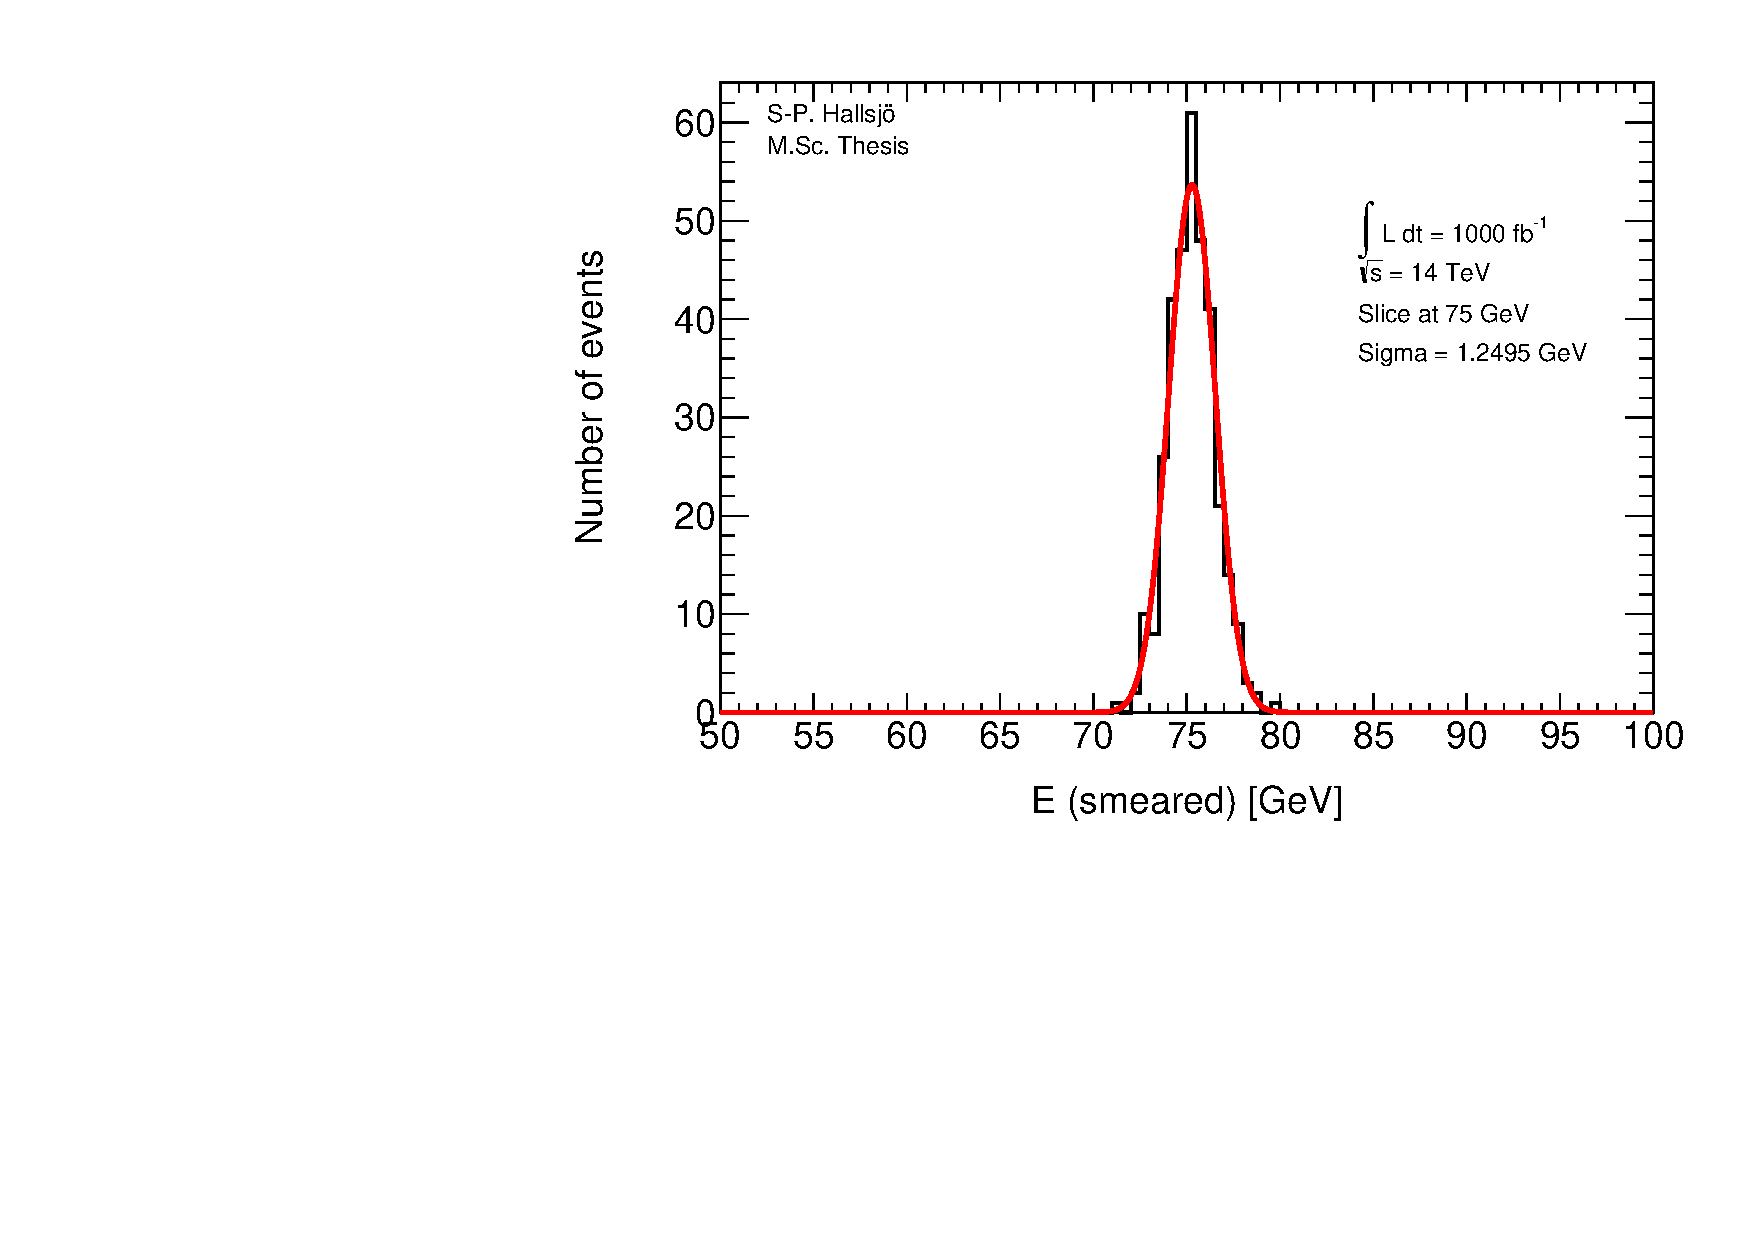
\includegraphics[width=0.5\textwidth]{eleta1.pdf}}% 
%\hfill
%  \subfloat[eleta2.\label{fig:elph:2}]{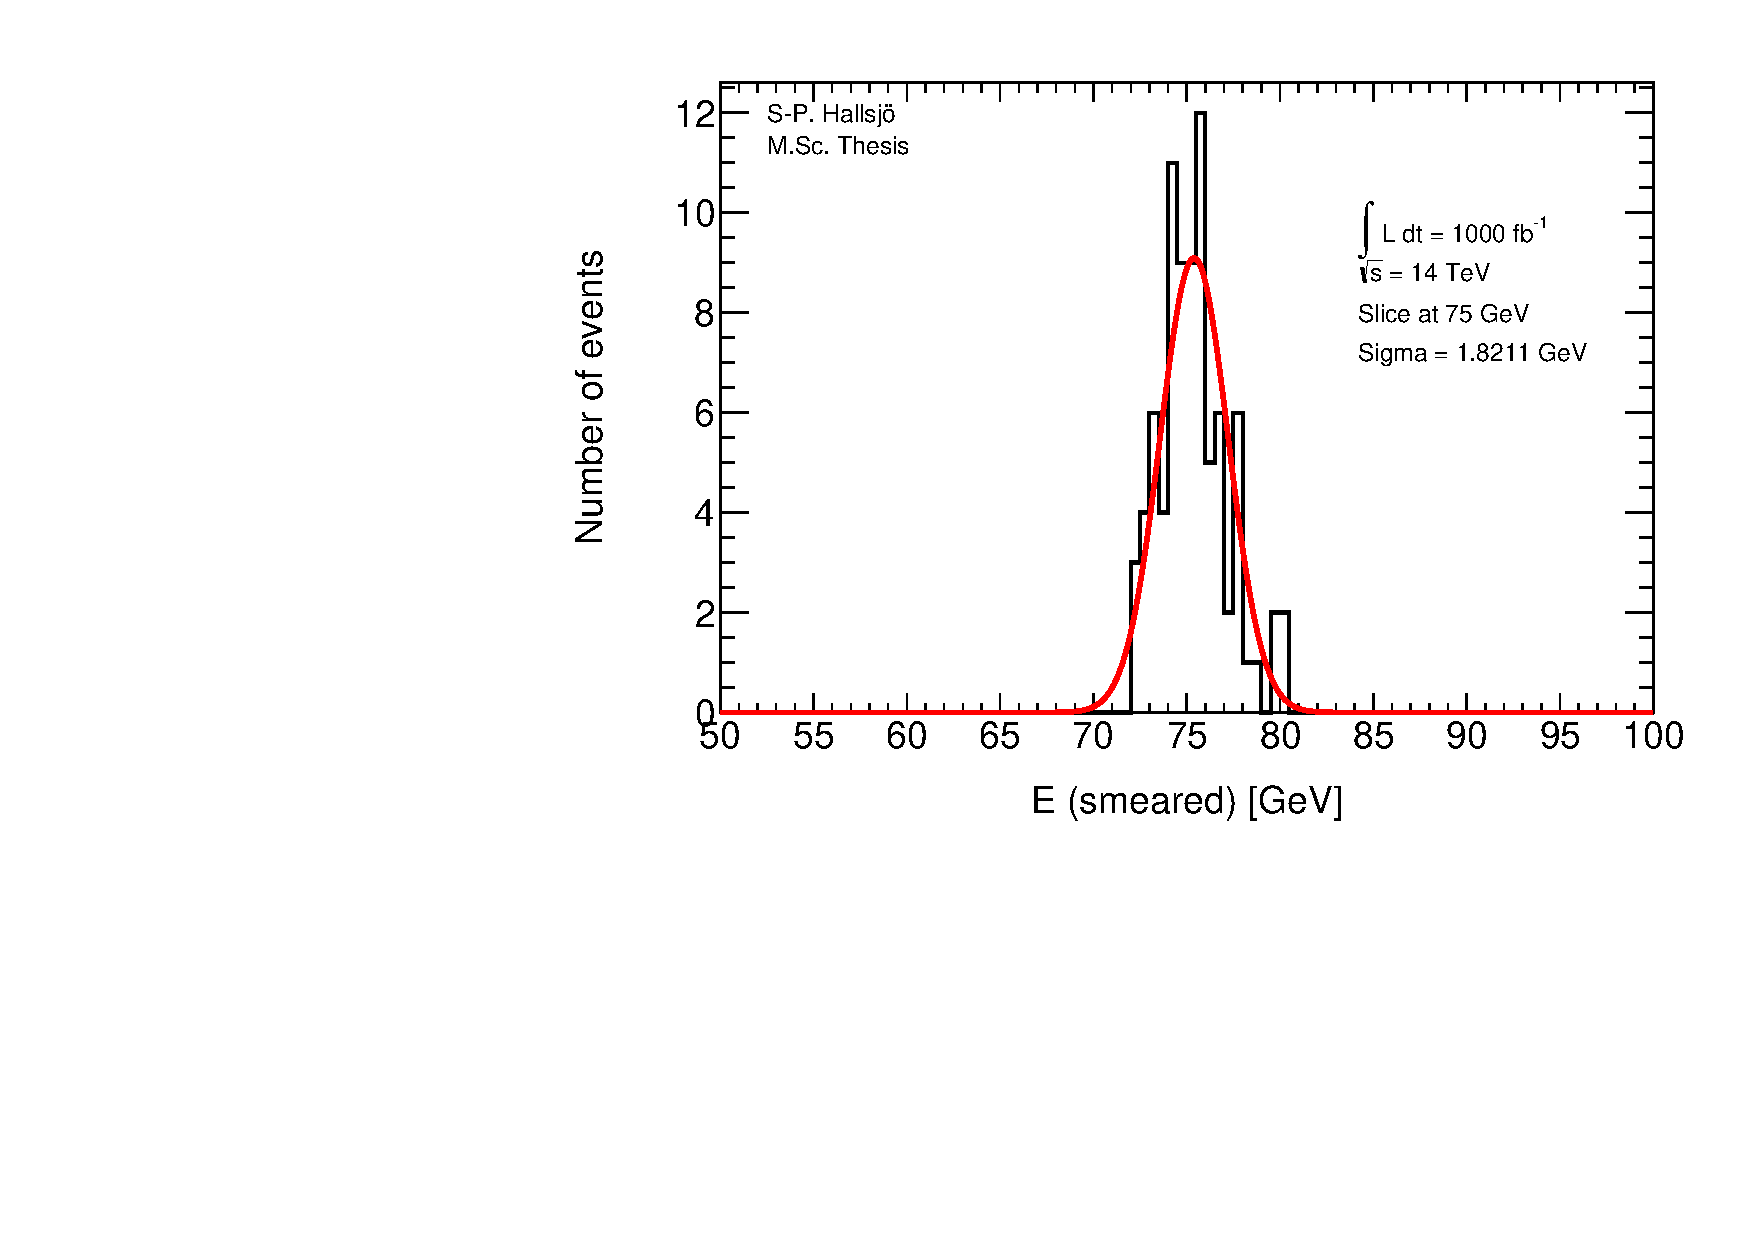
\includegraphics[width=0.5\textwidth]{eleta2.pdf}} 
%  \caption{el and ph eta}
%  \label{fig:elph}
%\end{figure}

%\begin{figure}[!htbp]
%% If it needs to be split.
%  \ContinuedFloat 
%  \centering 
%  \subfloat[pheta1. \label{fig:elph:3}]{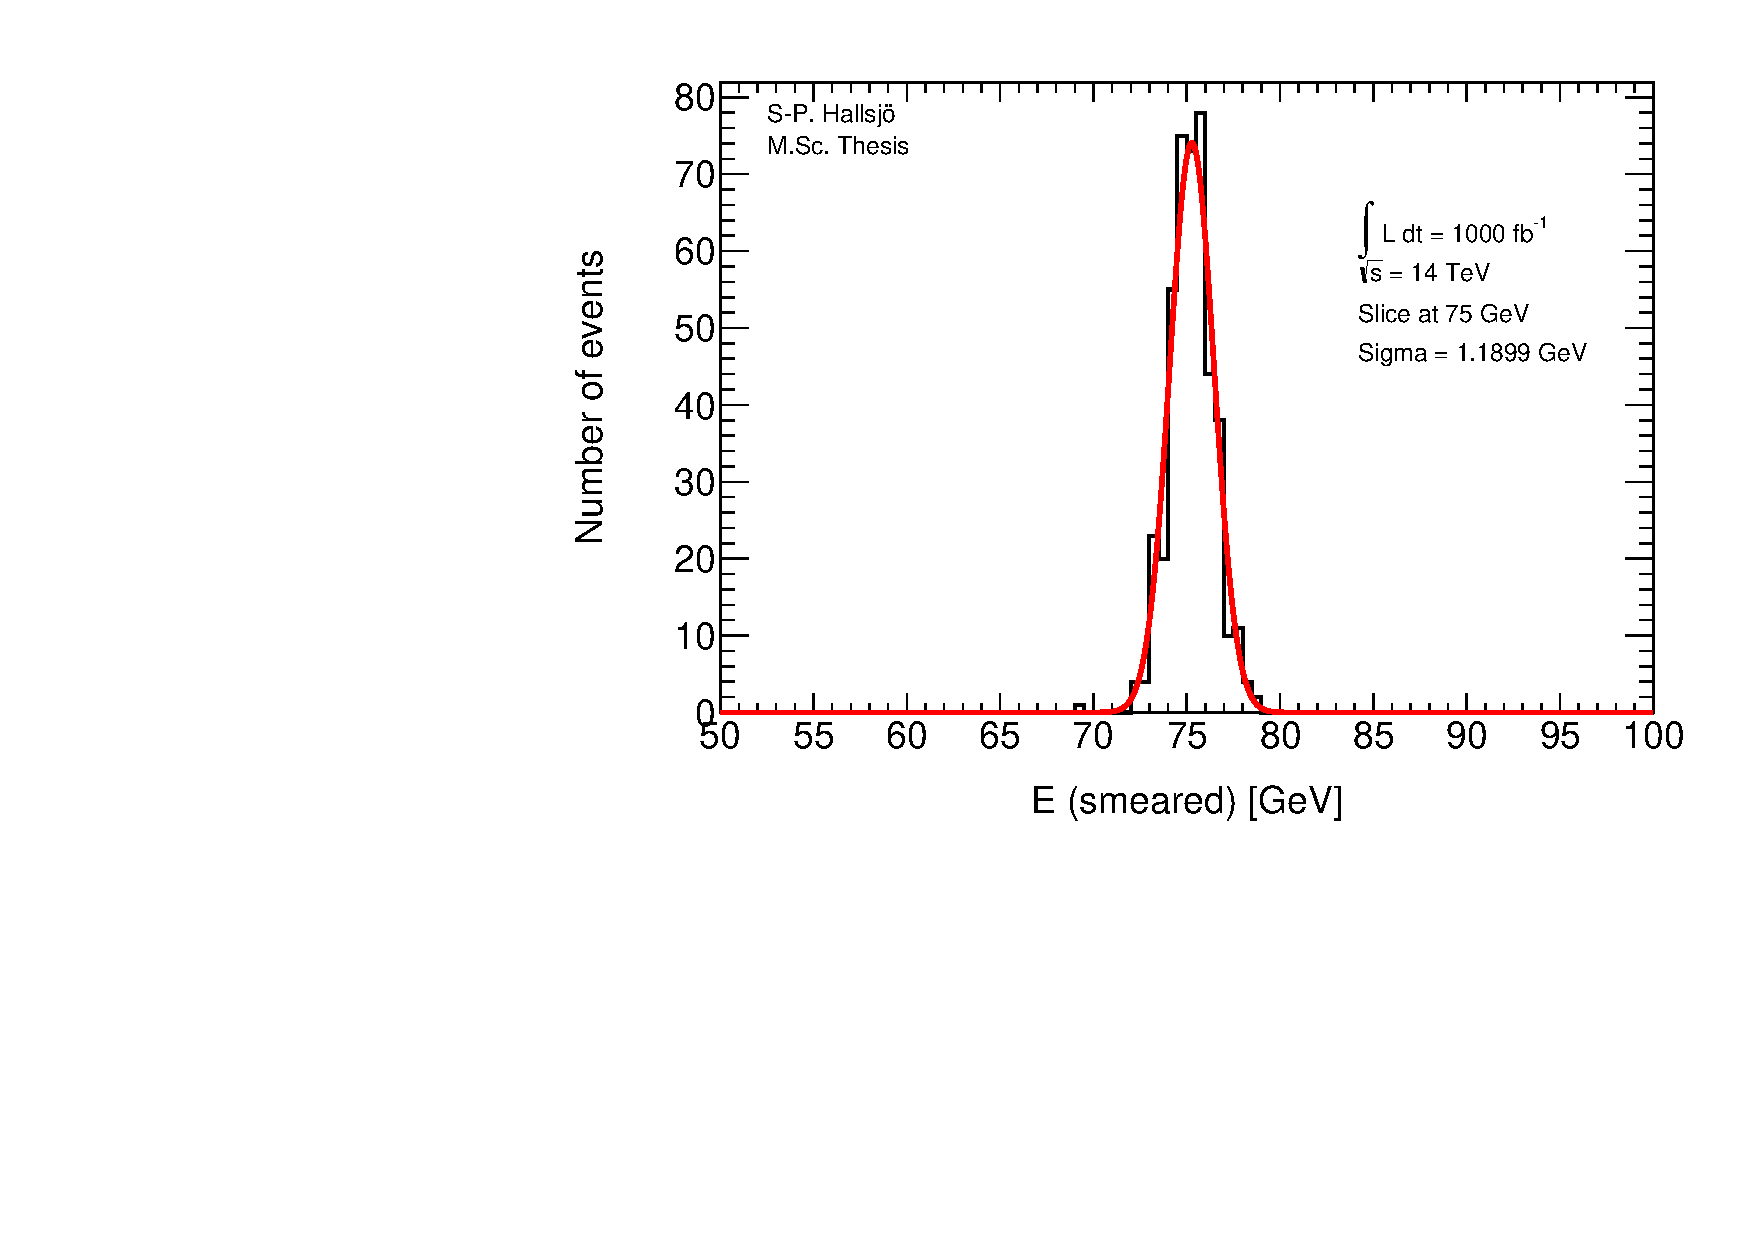
\includegraphics[width=0.5\textwidth]{pheta1.pdf}}% 
%  \hfill
%  \subfloat[pheta2.\label{fig:elph:4}]{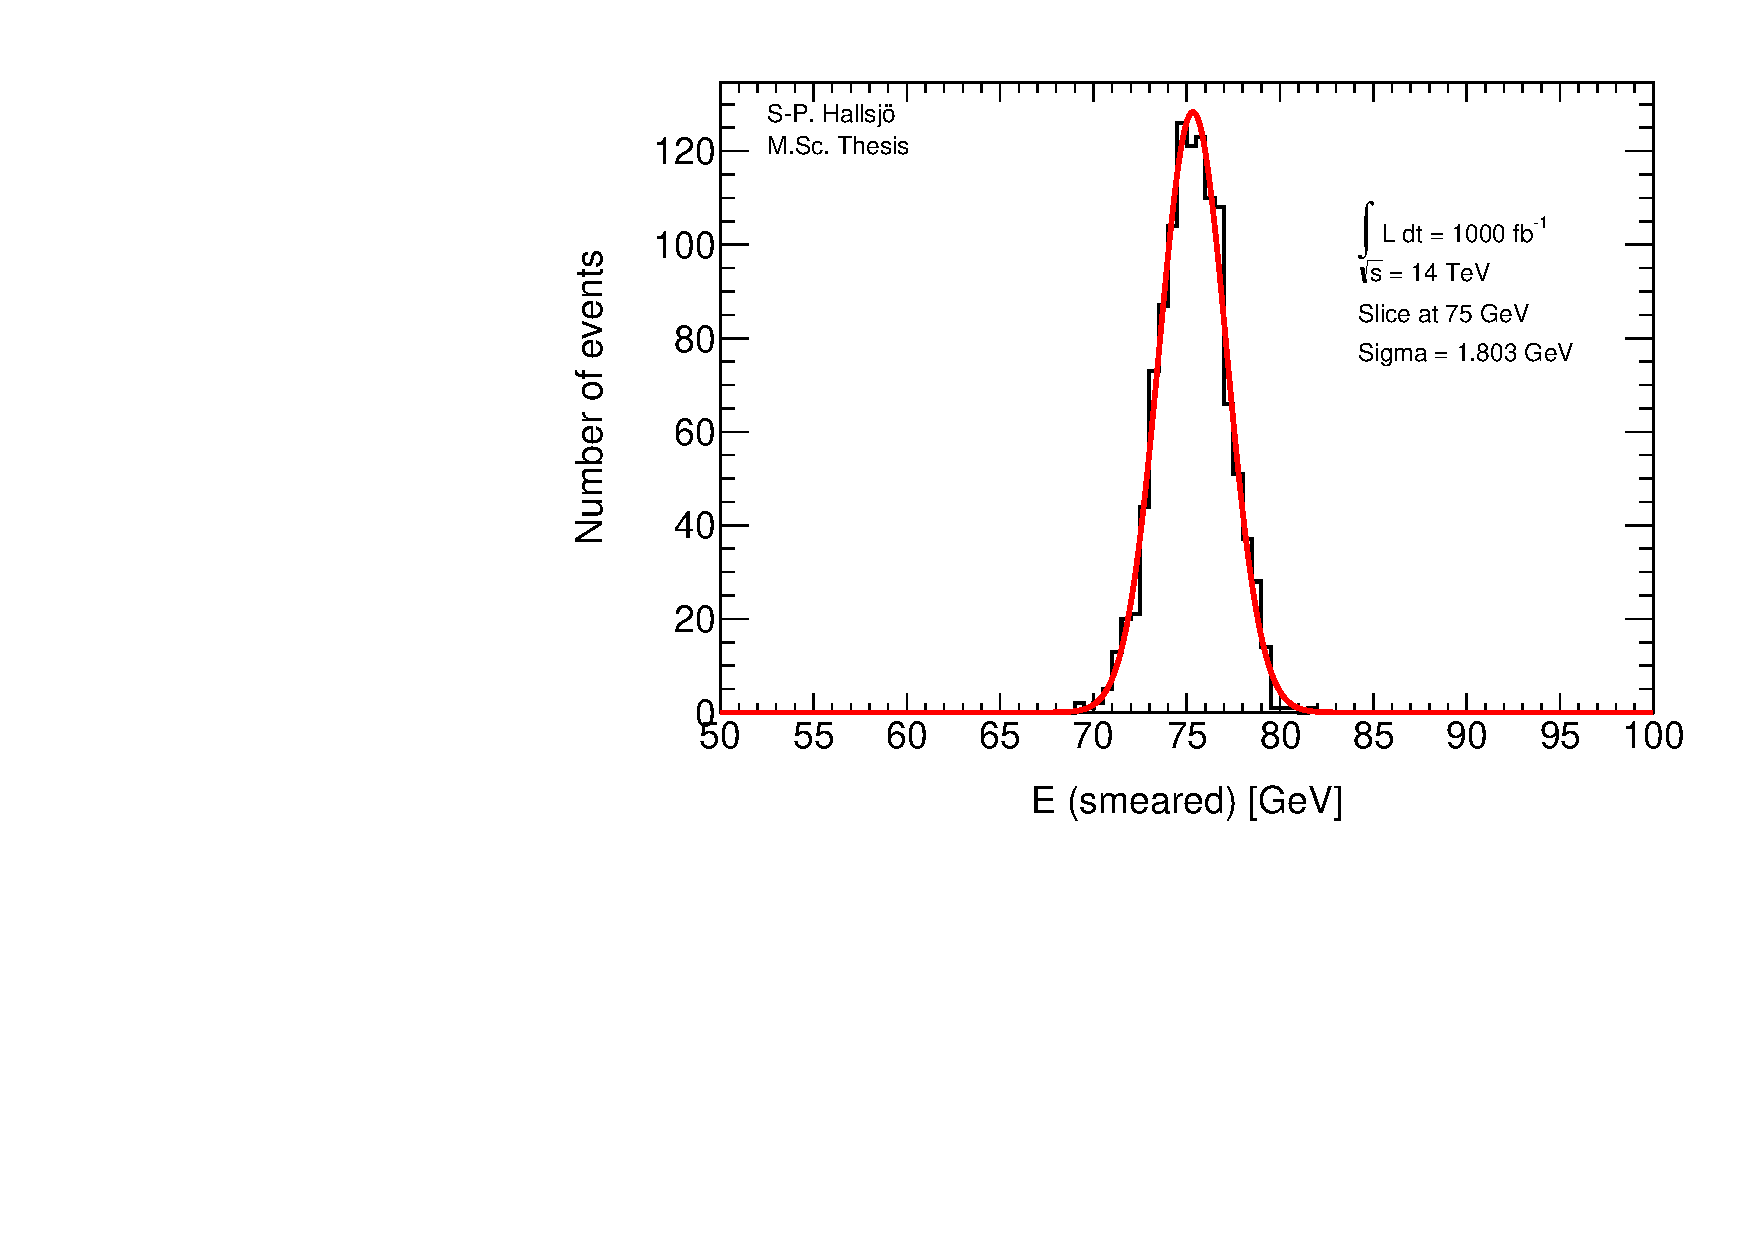
\includegraphics[width=0.5\textwidth]{pheta2.pdf}} 
%  \setcounter{figure}{1}
%  \caption[]{el and ph eta}
%  \label{fig:elph}
%\end{figure} 
%\setcounter{figure}{1}

 \begin{figure}[H] %!ht
    \subfloat[Electron energy after smearing for $\abs{\eta}<1.4$. \label{fig:elph:1}]{%
    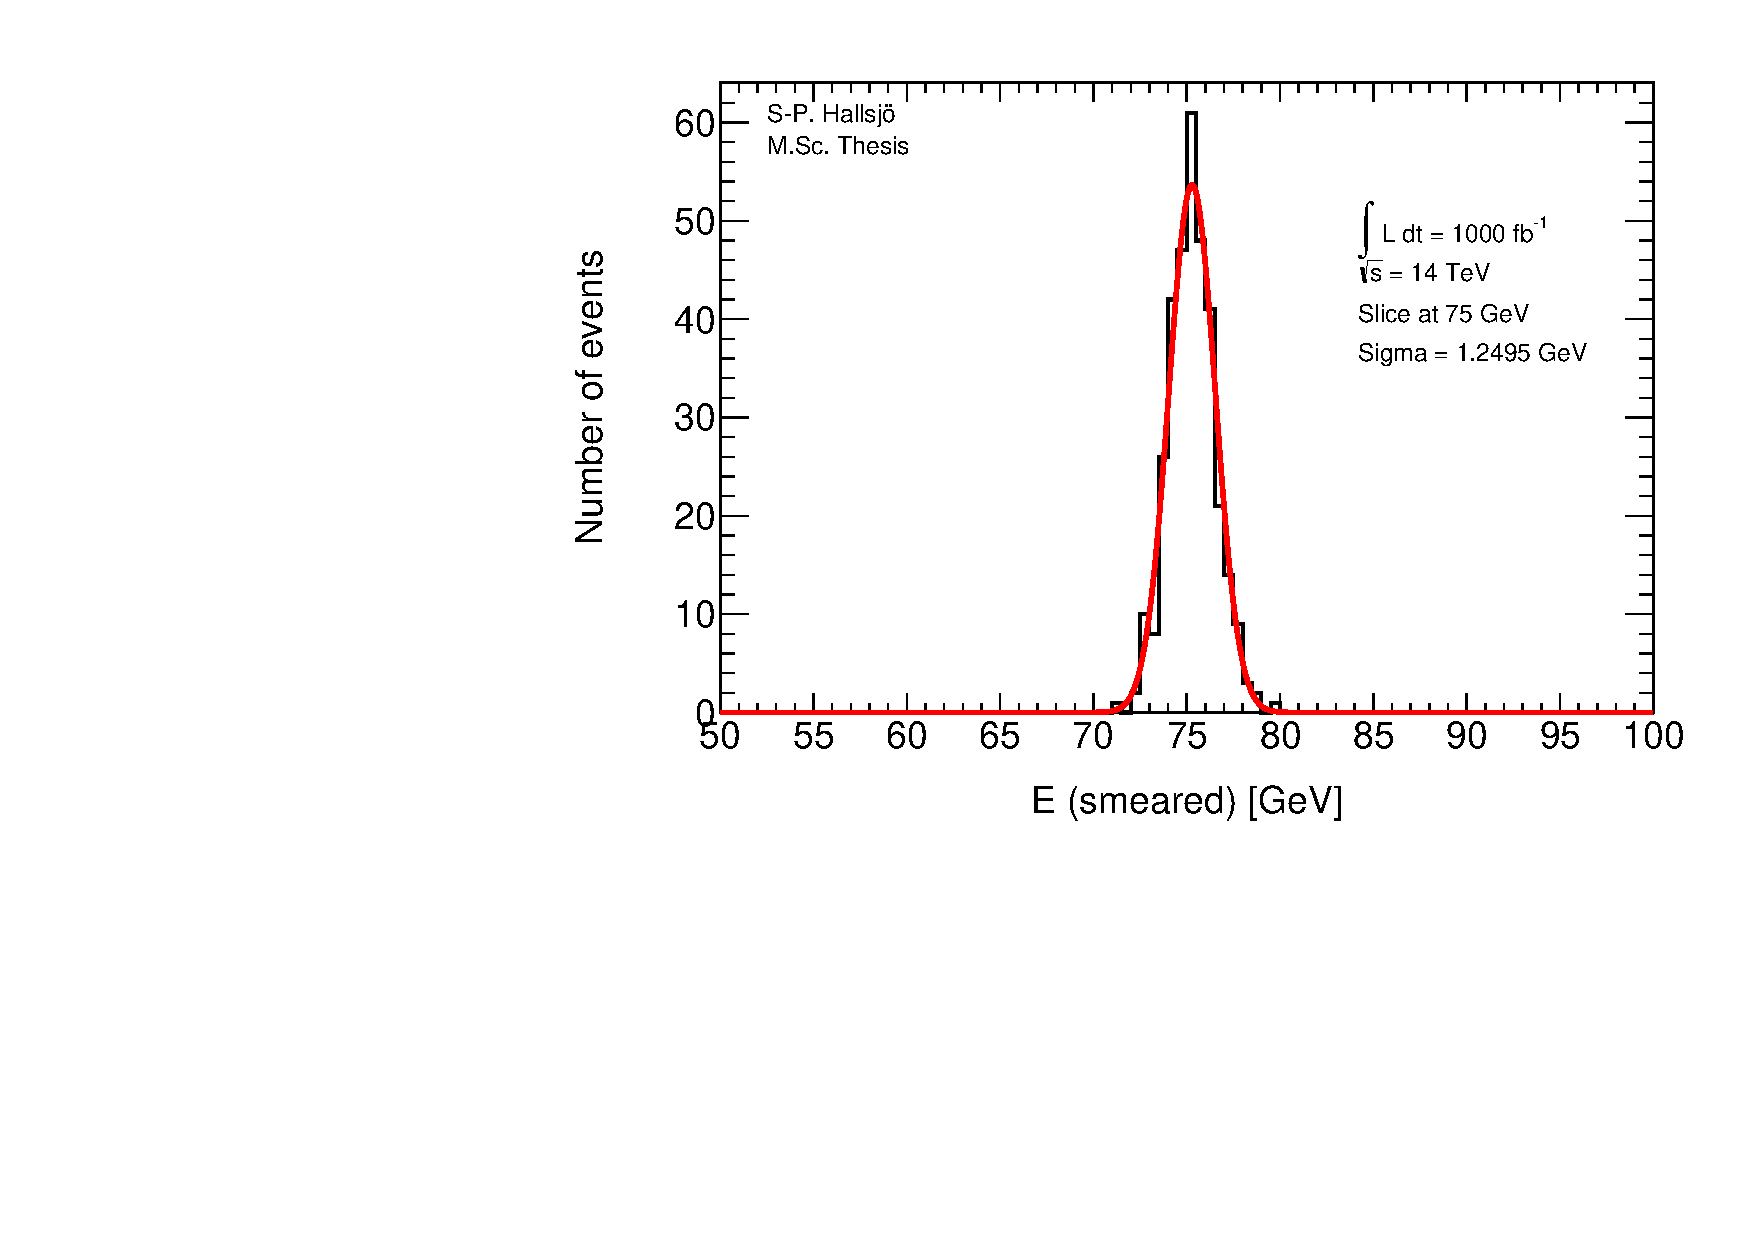
\includegraphics[width=0.5\textwidth]{eleta1.pdf}
    }
    \hfill
\subfloat[Electron energy after smearing for $1.4<\abs{\eta}<2.47$.\label{fig:elph:2}]{%
      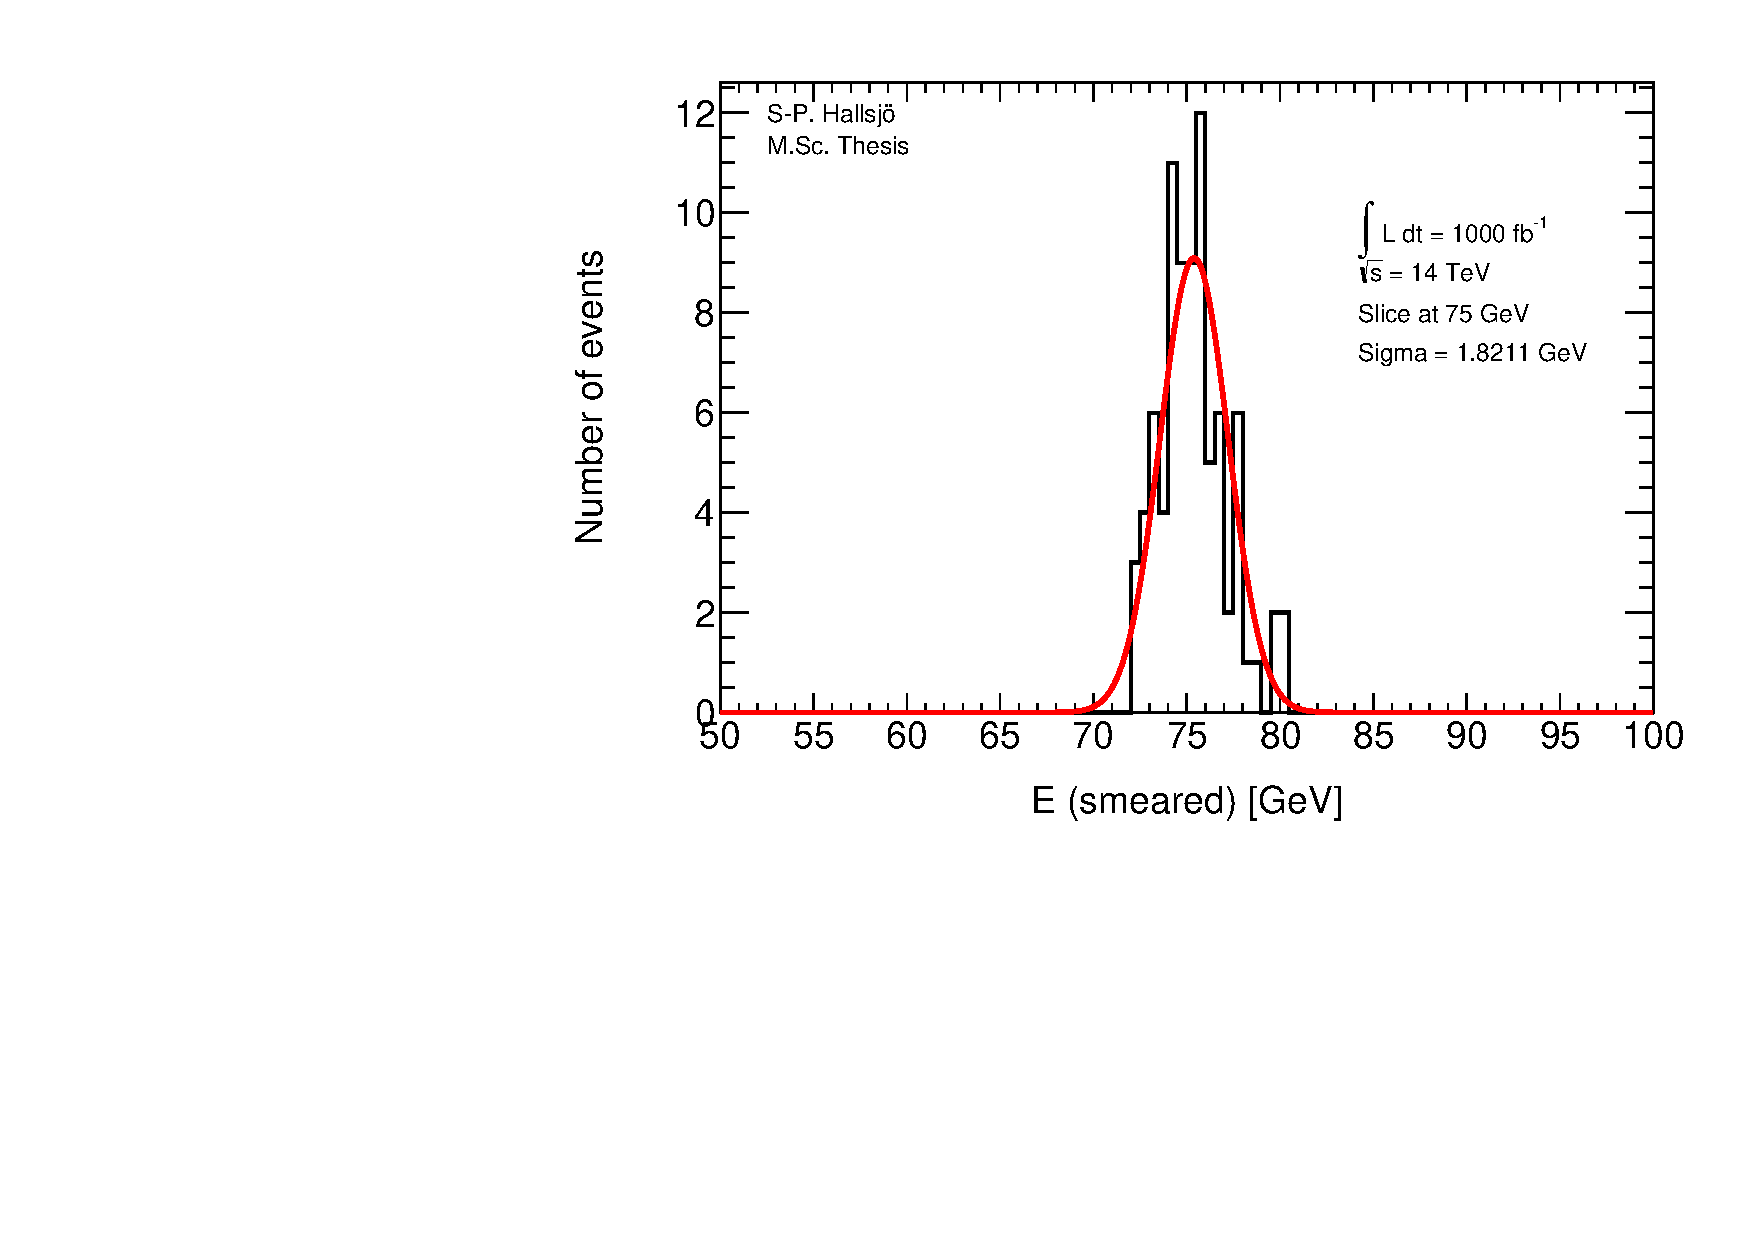
\includegraphics[width=0.5\textwidth]{eleta2.pdf}
    }
    \hfill
        \subfloat[Photon energy after smearing for $\abs{\eta}<1.4$. \label{fig:elph:3}]{%
     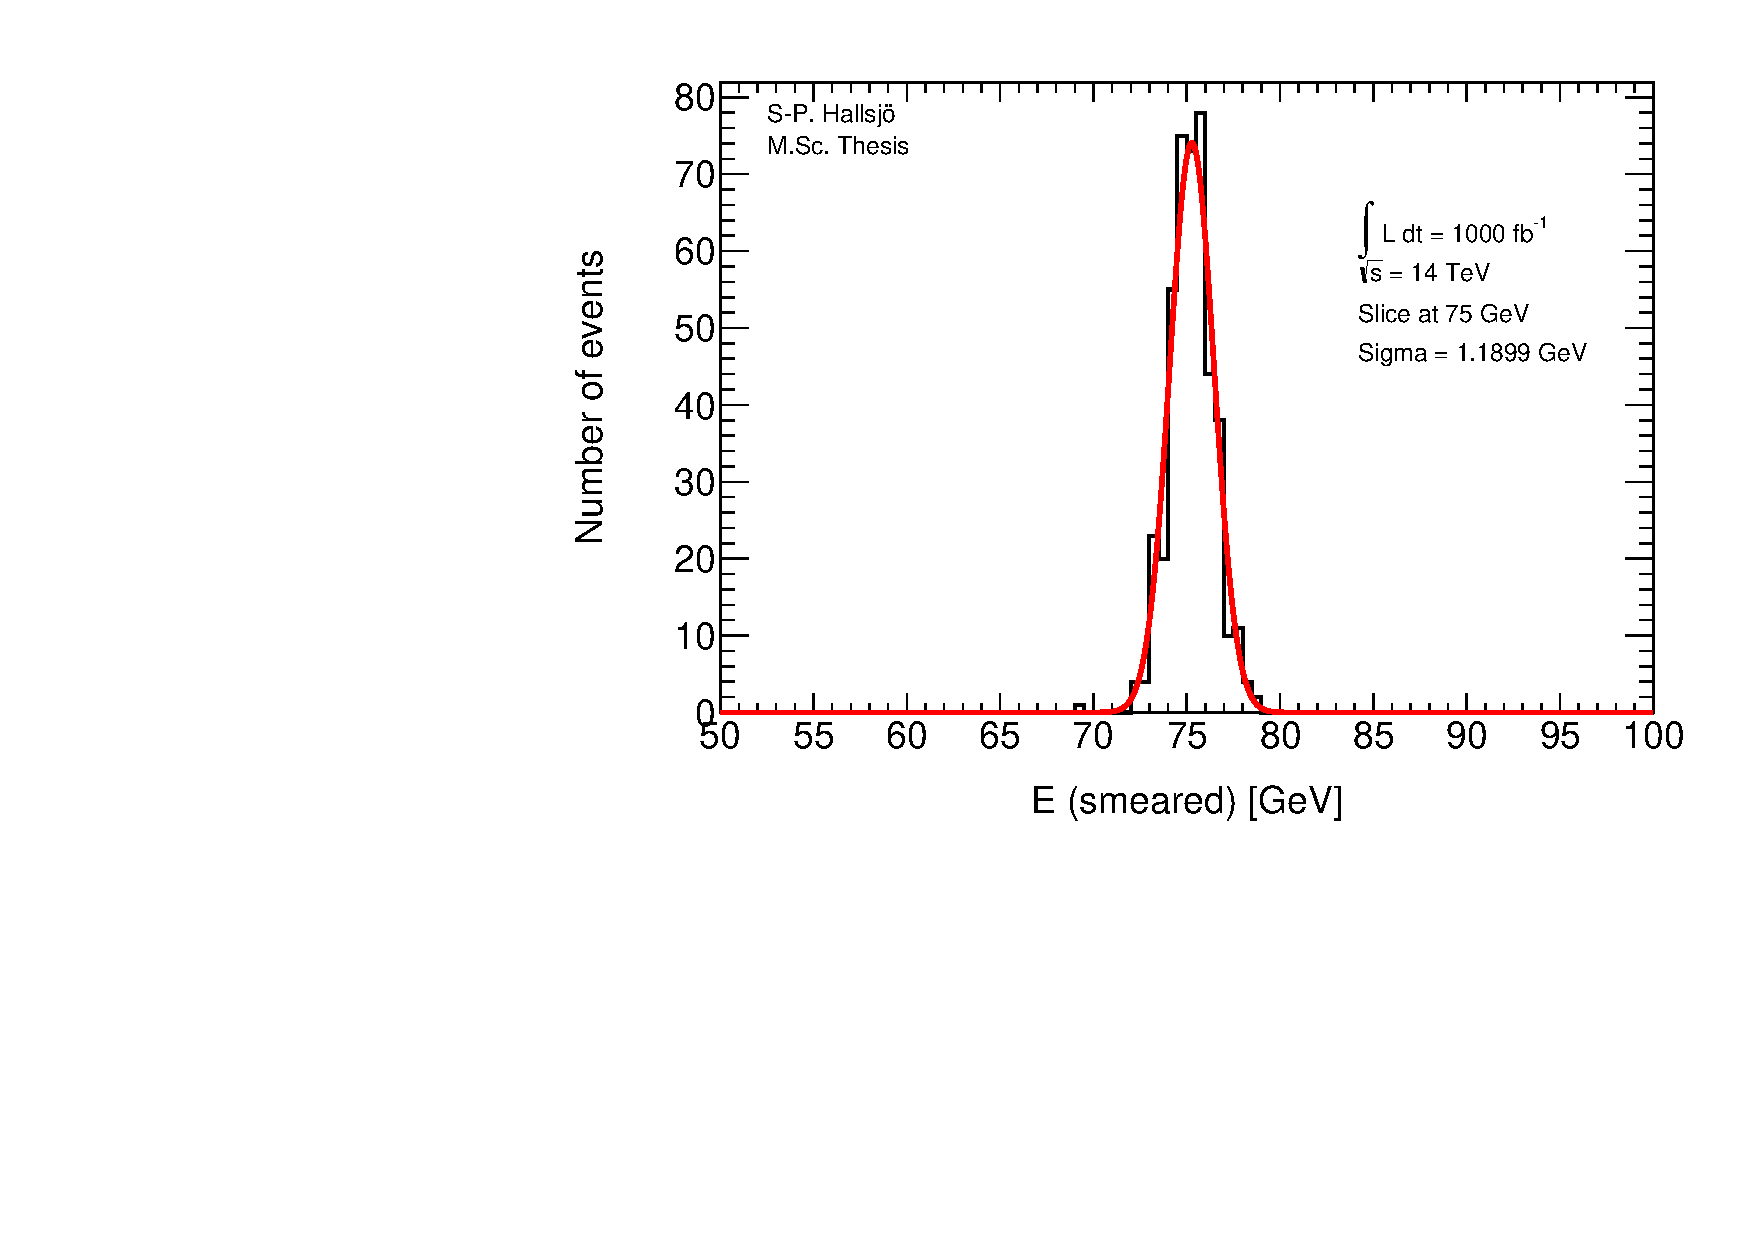
\includegraphics[width=0.5\textwidth]{pheta1.pdf}
    }
    \hfill
\subfloat[Photon energy after smearing for $1.4<\abs{\eta}<2.47$.\label{fig:elph:4}]{%
     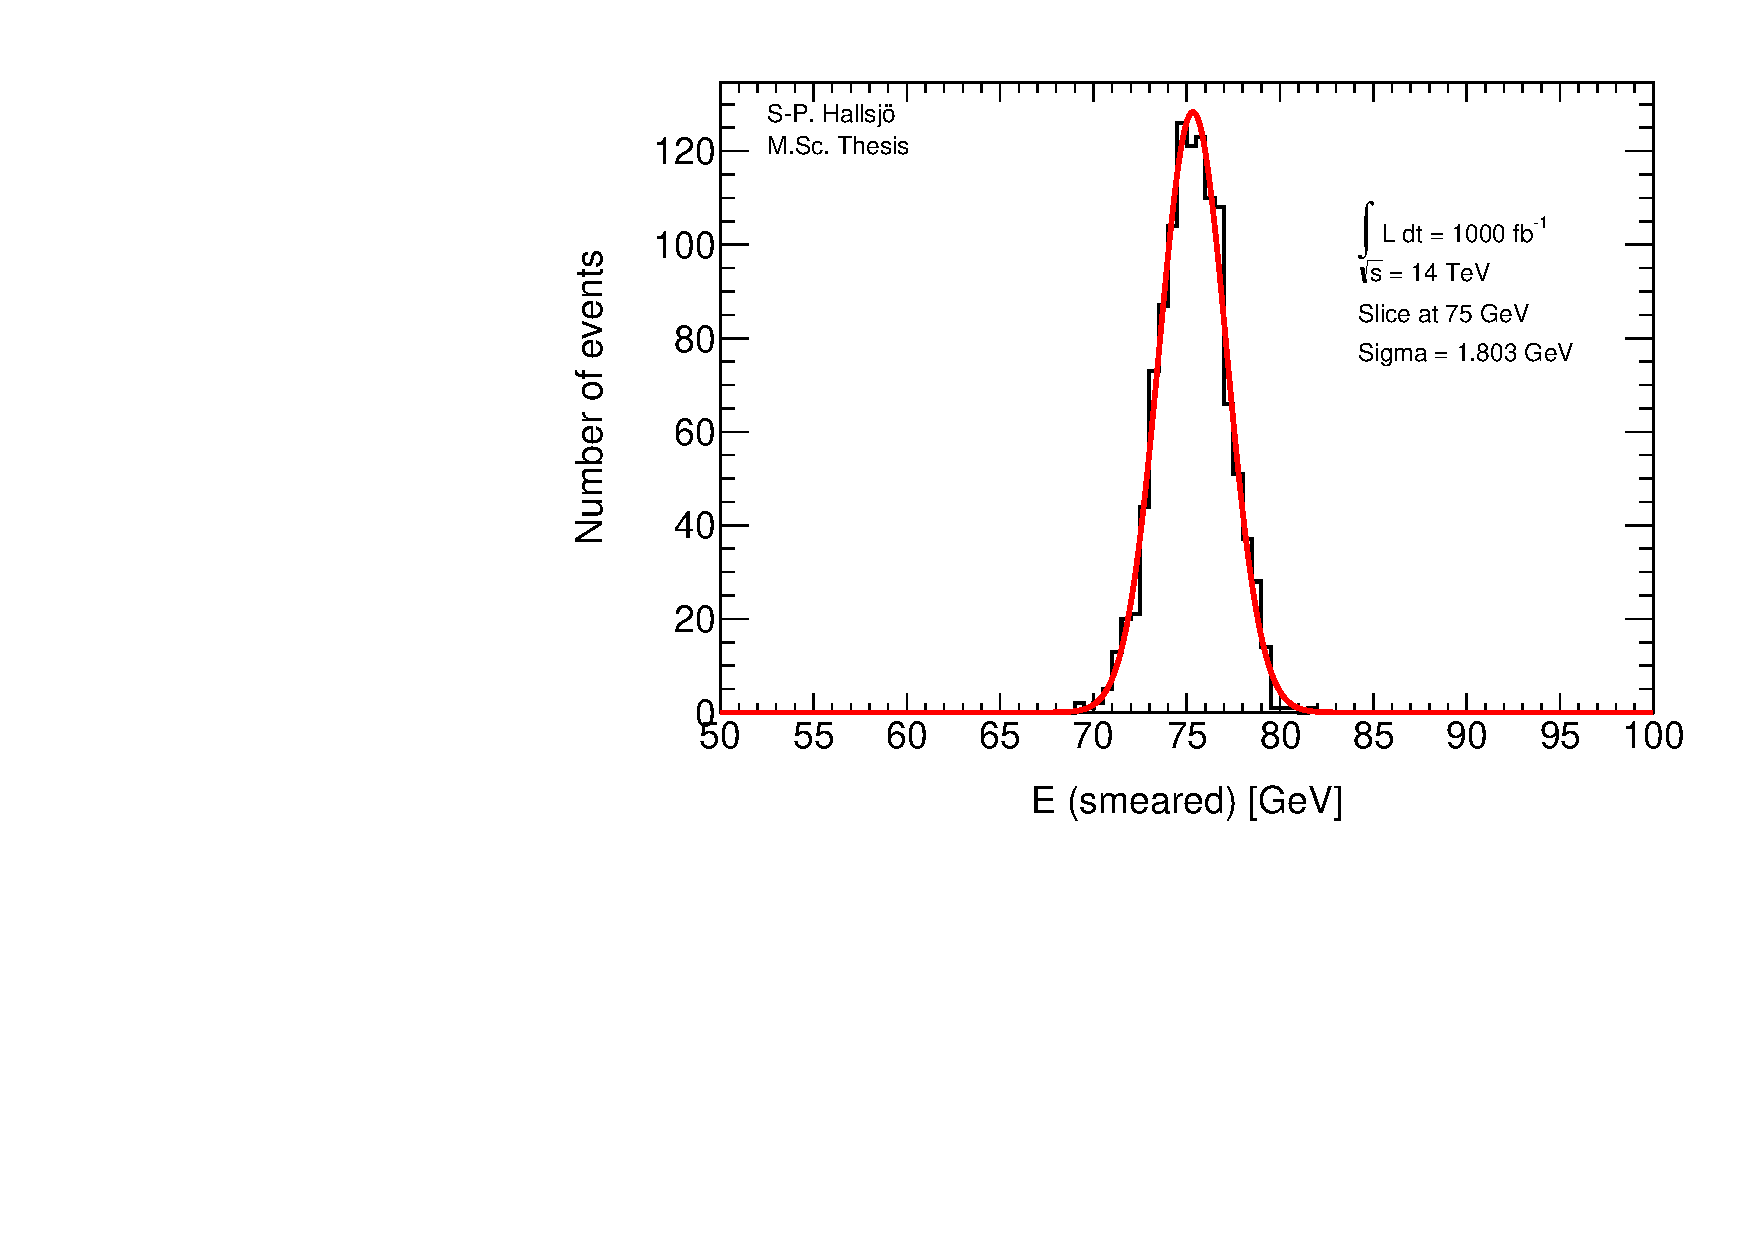
\includegraphics[width=0.5\textwidth]{pheta2.pdf}
    }
    \caption{Photon and electron energy after smearing.}
    \label{fig:elph}
\end{figure}
\newpage
\subsection{Muon}
Since muons detection is shielded from the effects of pile-up only efficiency and detector limitations affect the smearing. In \figureref{fig:muon} the Gaussian fit (red) and the data (black) are given for the muon momenta.
 \begin{figure}[H] %!ht
    \subfloat[Muon momenta after smearing for $\abs{\eta}<1.05$. \label{fig:muon:1}]{%
     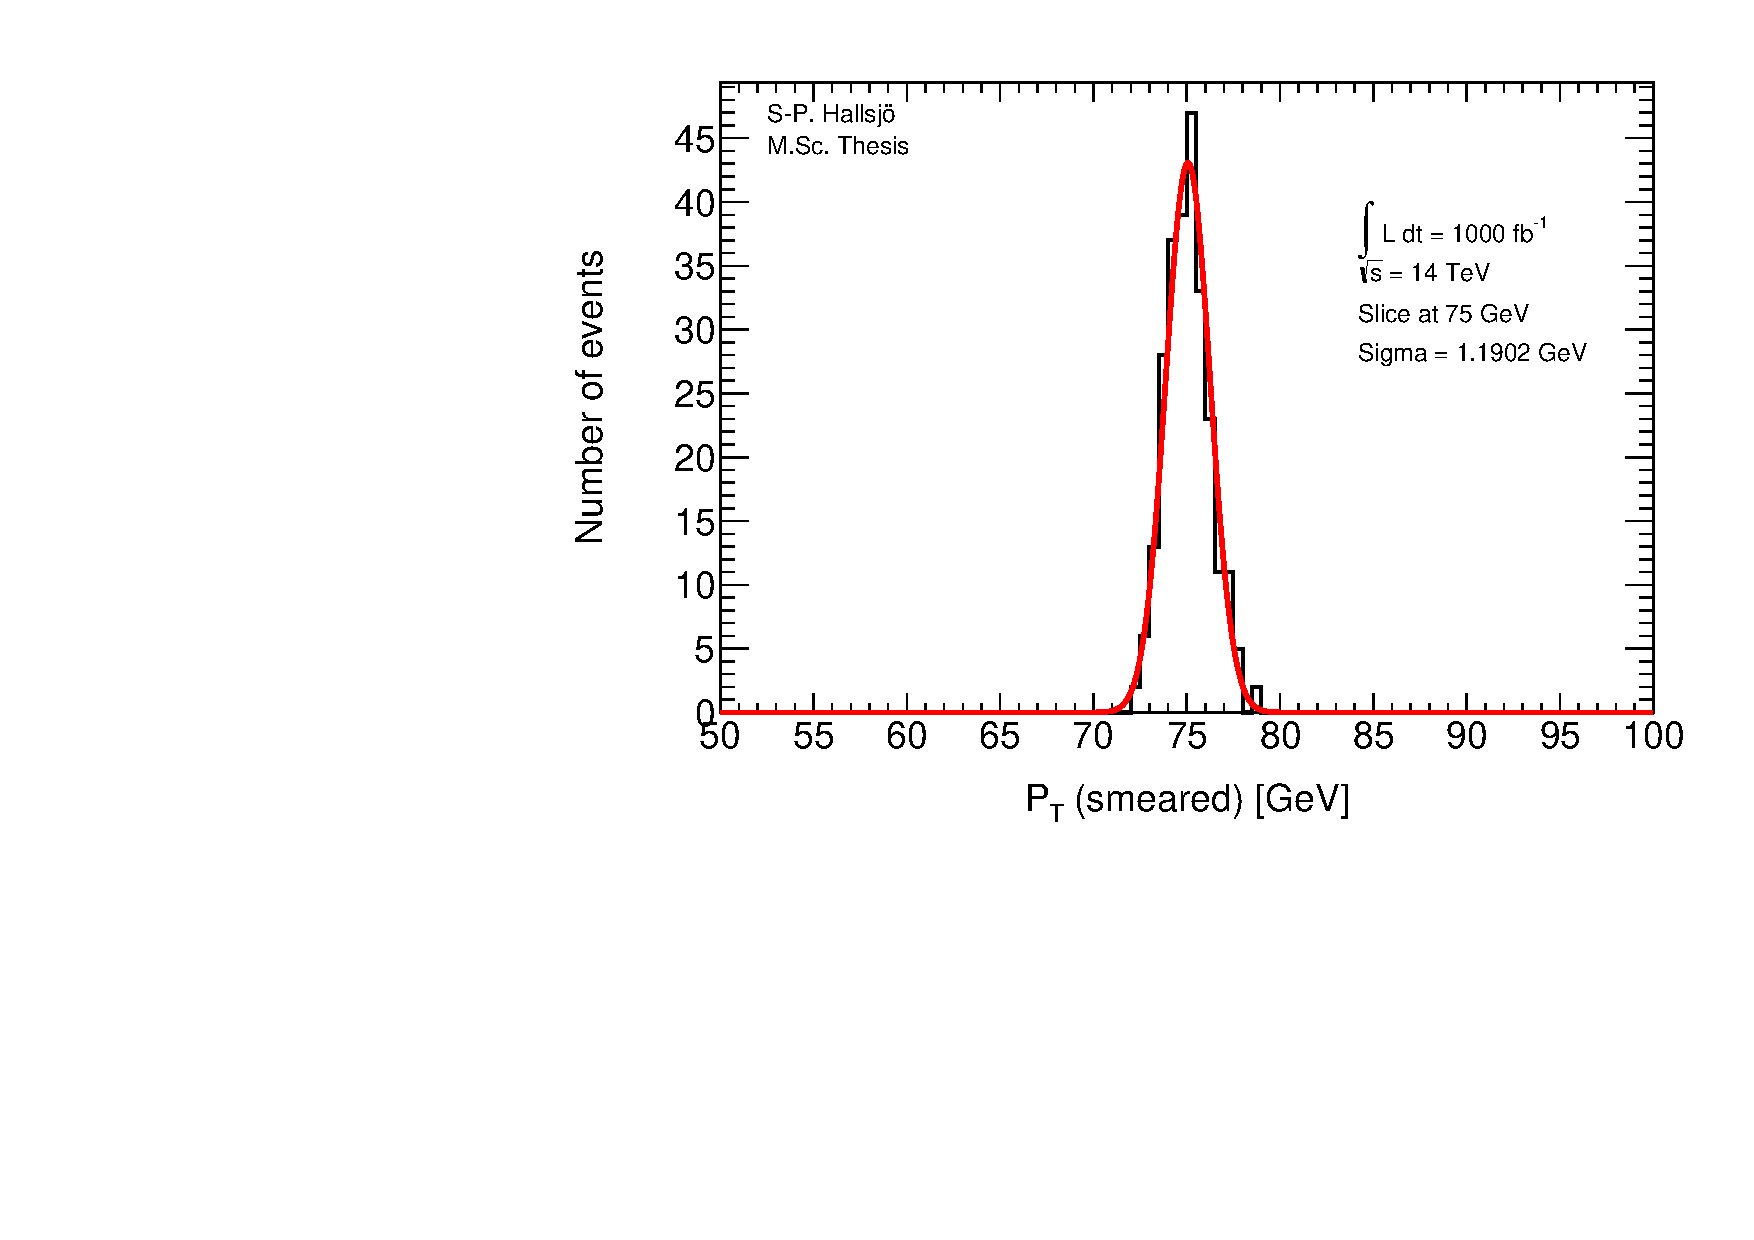
\includegraphics[width=0.5\textwidth]{mueta1.pdf}
    }
    \hfill
    \subfloat[Muon momenta after smearing for $1.05<\abs{\eta}$.\label{fig:muon:2}]{%
      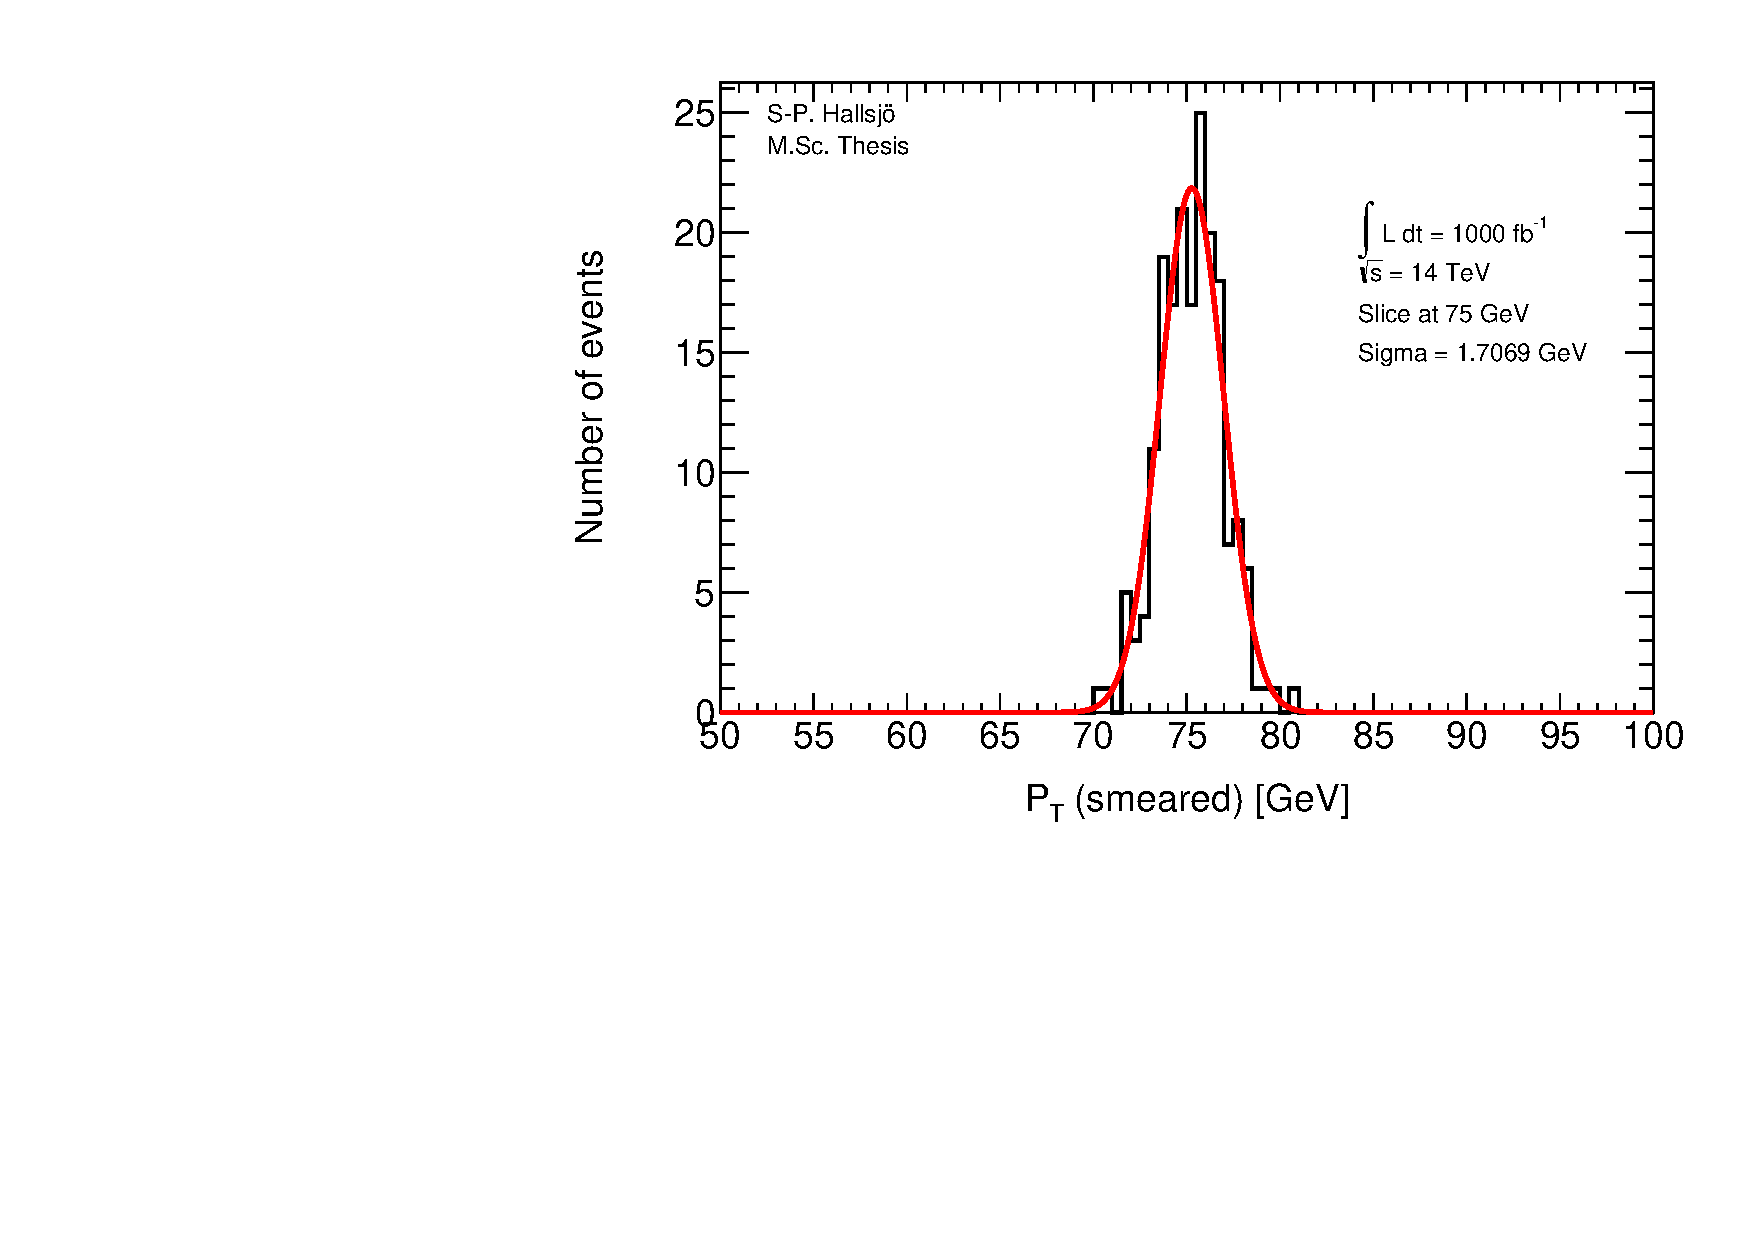
\includegraphics[width=0.5\textwidth]{mueta2.pdf}
    }
    \caption{Muon momenta after smearing.}
    \label{fig:muon}
  \end{figure}
\subsection{Tau}
As described in \subsectionref{sec:smear:subsec:tau} tauons are detected similarly to electrons and photons. Thus the plots should look similarly to those in the previous subsection apart from the peak value being at 150 GeV. In \figureref{fig:tau:1} the Gaussian fit (red) and the data (black) are given for tau detected through 3 prong. In \figureref{fig:tau:2} smeared energy is plotted against truth energy. 
 \begin{figure}[H] %!ht
    \subfloat[Tau energy after smearing. \label{fig:tau:1}]{%
     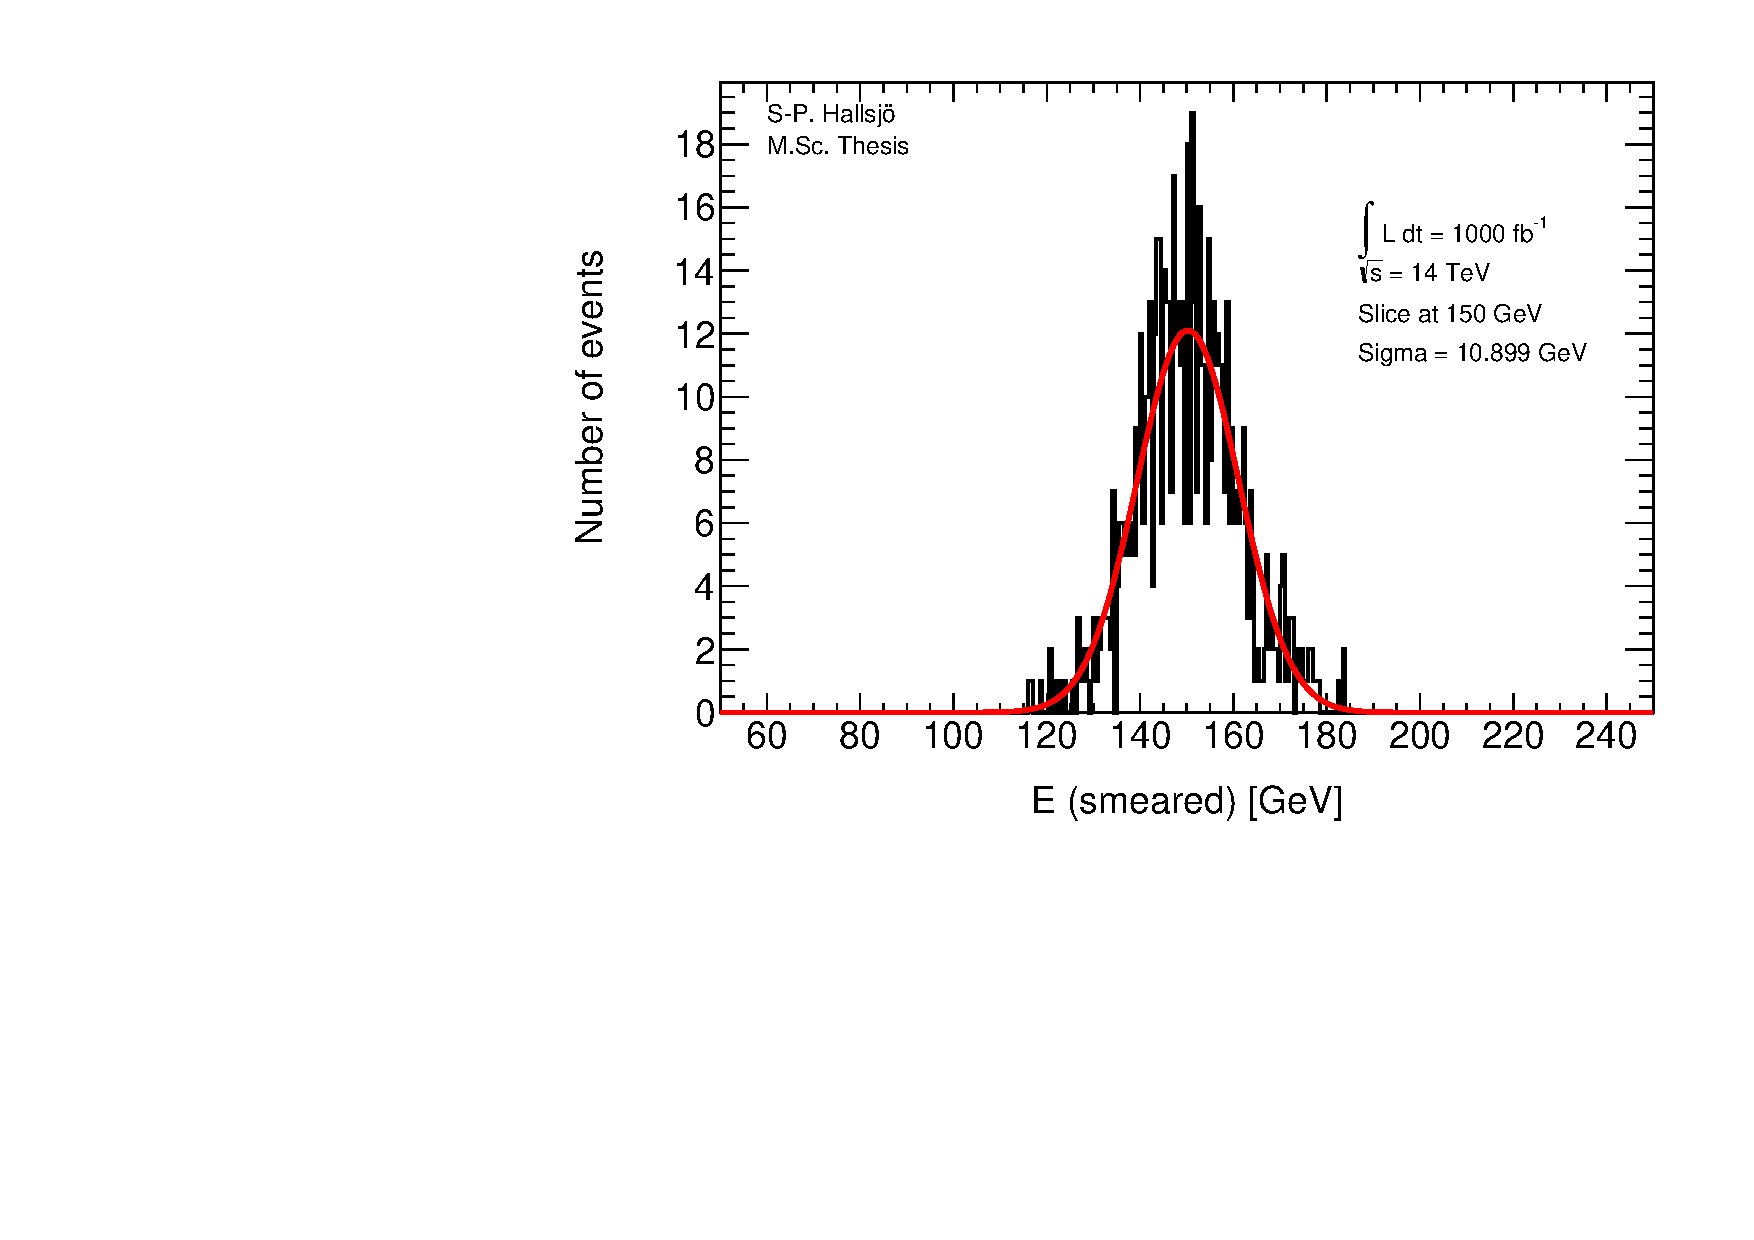
\includegraphics[width=0.5\textwidth]{tau.pdf}
    }
    \hfill
    \subfloat[Tau smeared vs truth. \label{fig:tau:2}]{%
      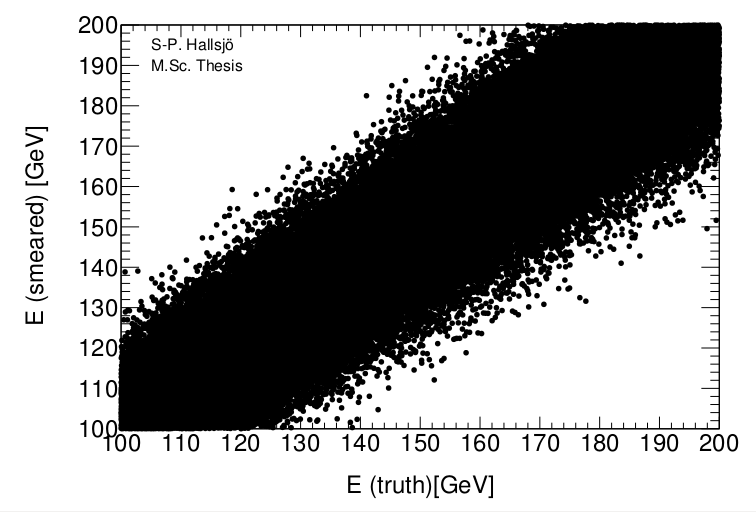
\includegraphics[width=0.5\textwidth]{tau2.png}
    }
    \caption{Tau energy after smearing and smeared vs truth.}
    \label{fig:tau}
  \end{figure}
  \newpage
\subsection{Jets}
The smearing functions are divided into four different regions depending on the angle $\eta$. 
 \begin{figure}[H] %!ht
    \subfloat[Jet momenta after smearing \newline for $\abs{\eta}<0.8$. \label{fig:jet:1}]{%
     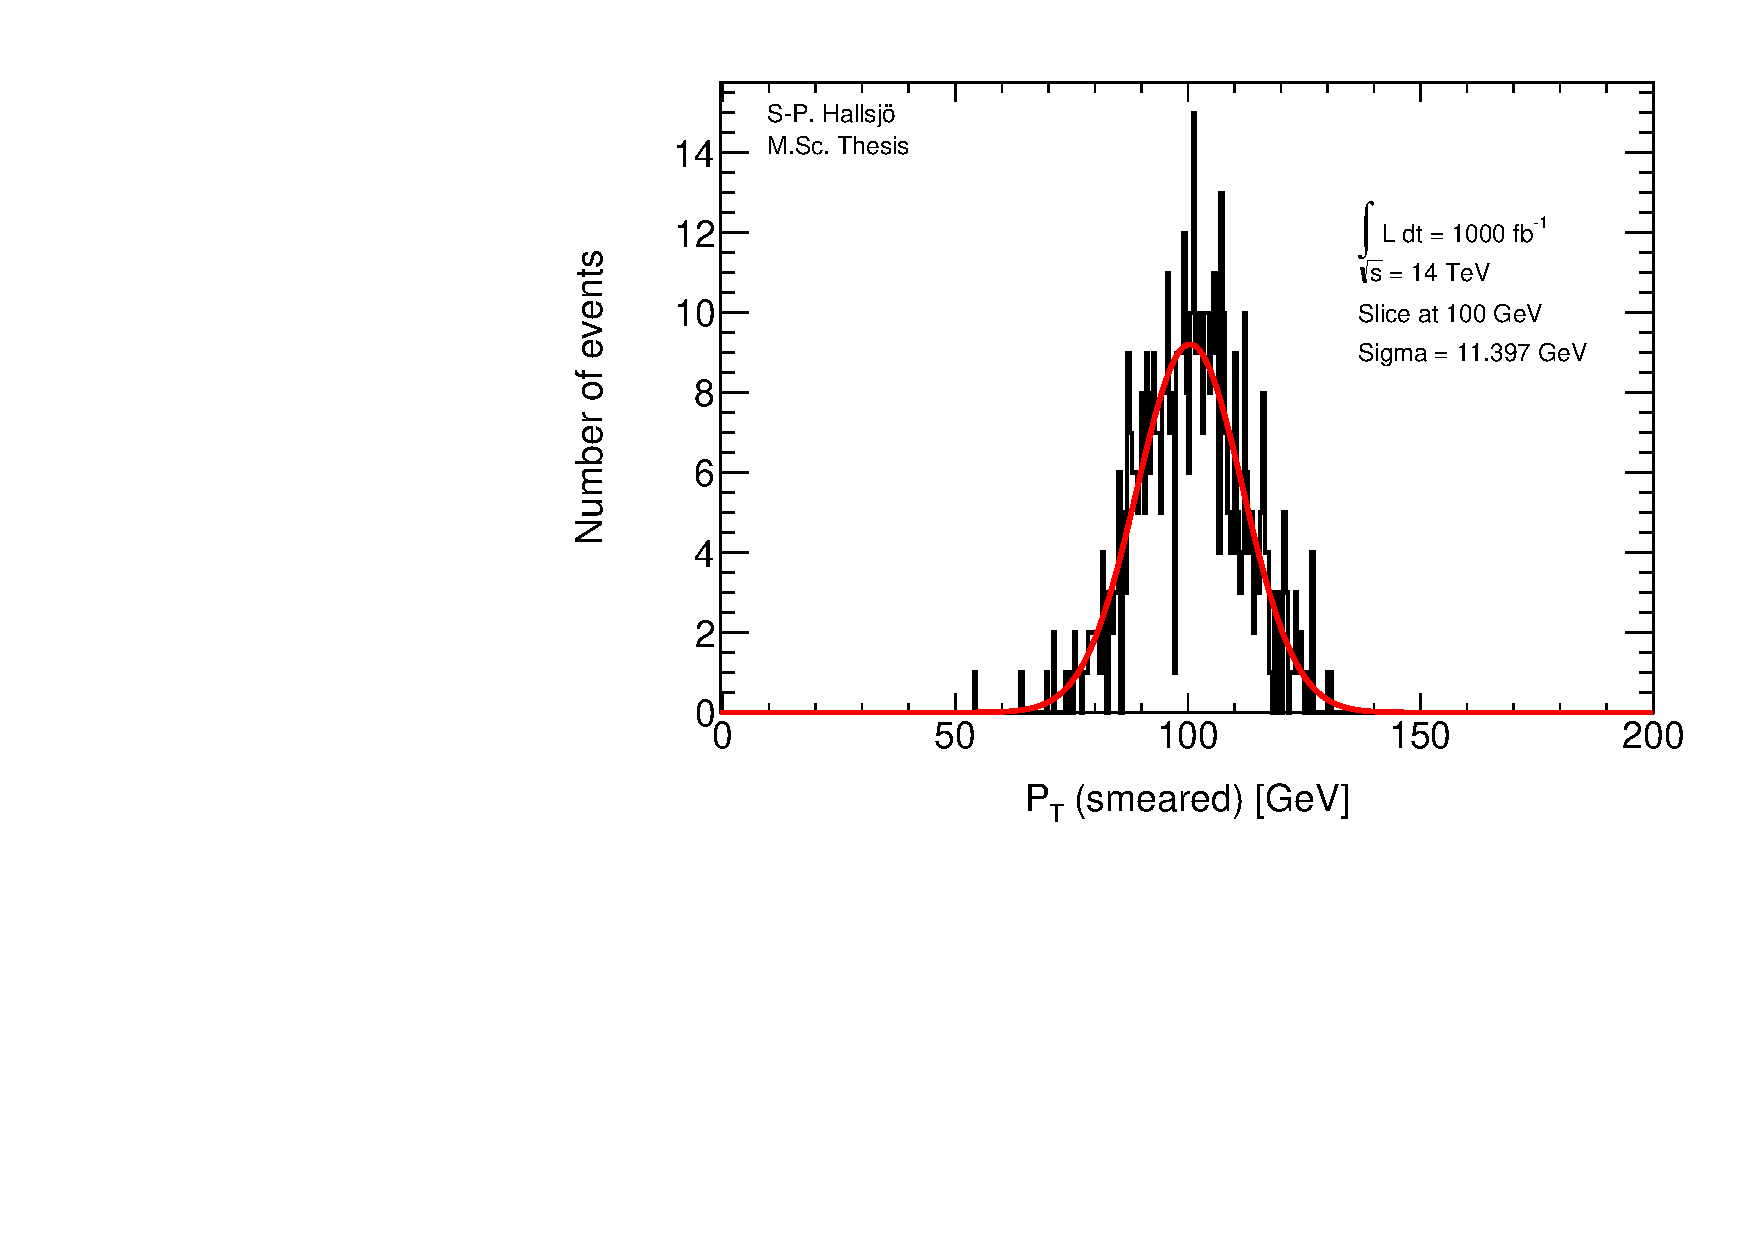
\includegraphics[width=0.5\textwidth]{jeteta1.pdf}
    }
    \hfill
\subfloat[For $0.8<\abs{\eta}<1.2$.\label{fig:jet:2}]{%
      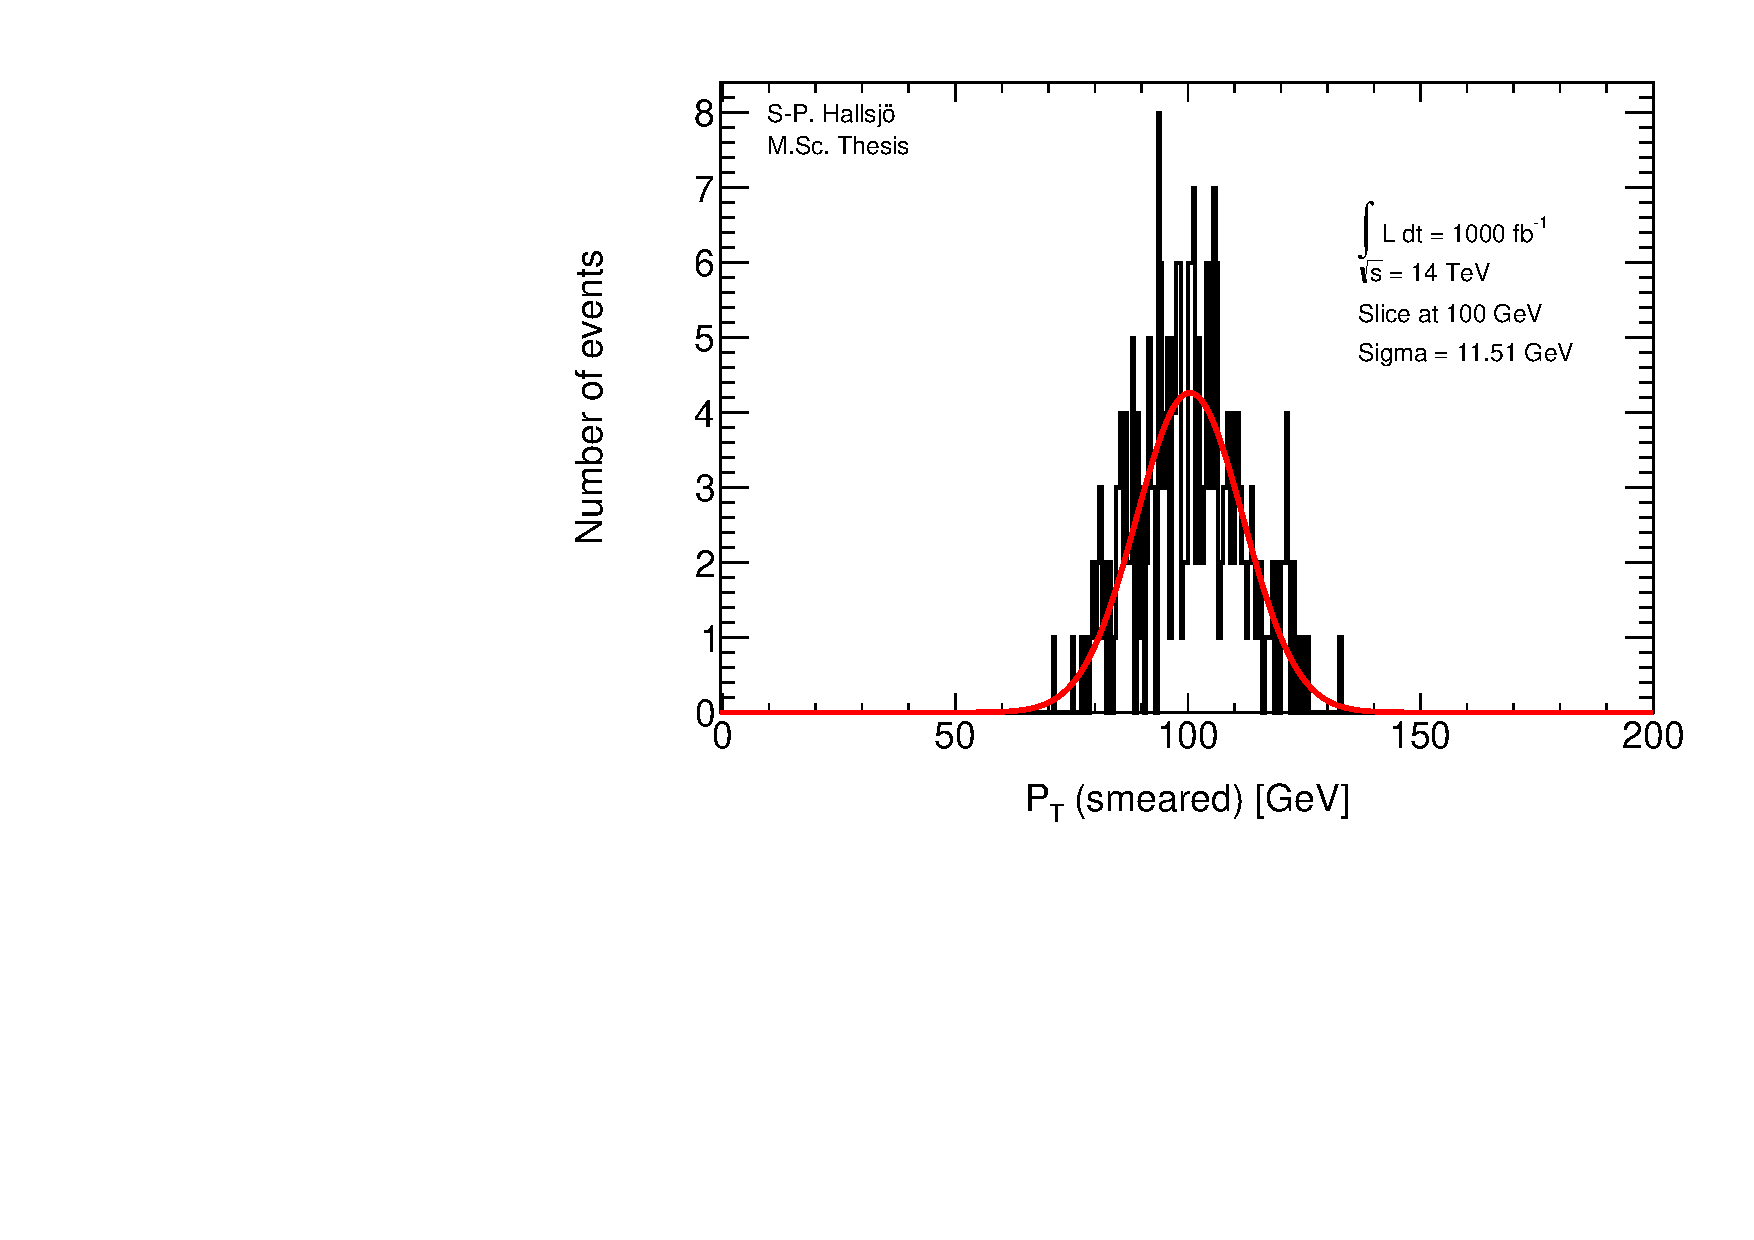
\includegraphics[width=0.5\textwidth]{jeteta2.pdf}
    }
    \hfill
        \subfloat[Jet momenta after smearing \newline for $1.2<\abs{\eta}<2.8$. \label{fig:jet:3}]{%
     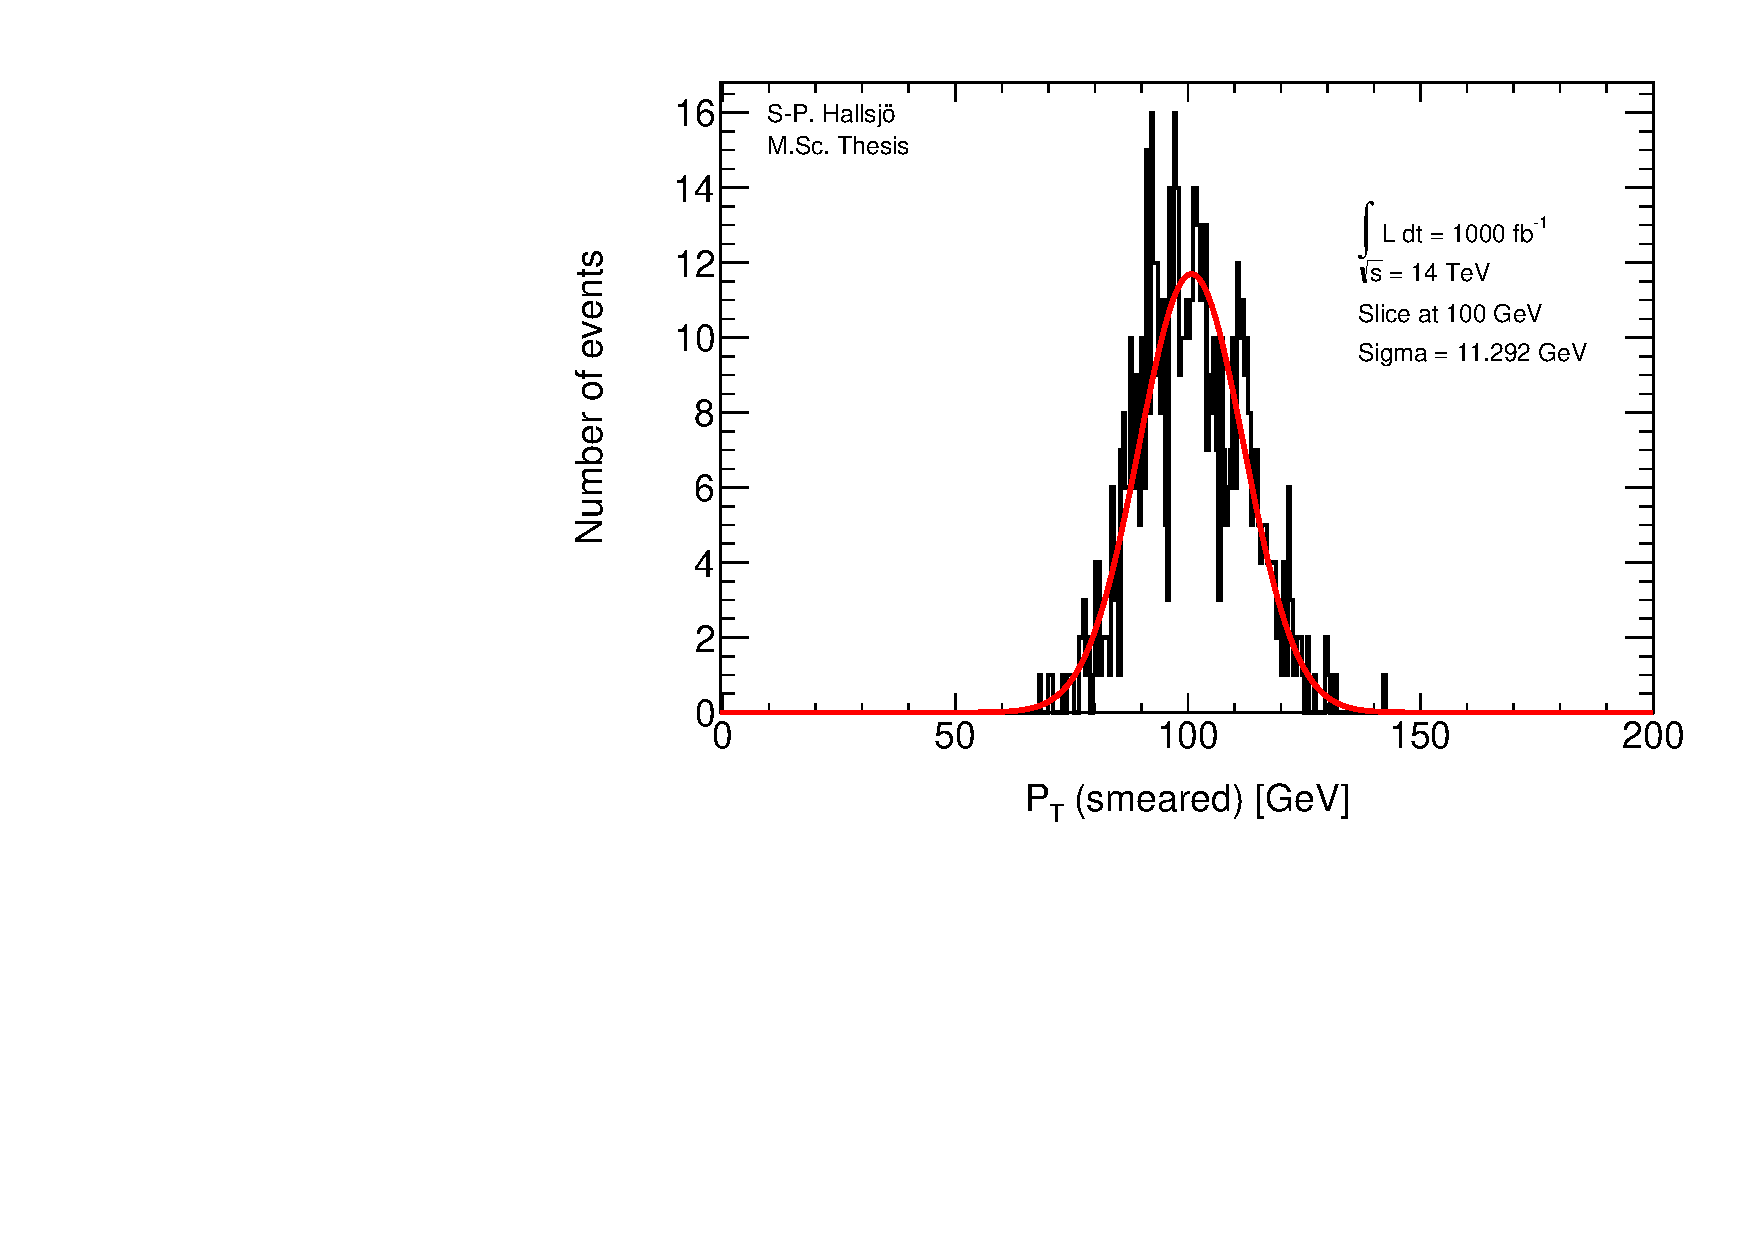
\includegraphics[width=0.5\textwidth]{jeteta3.pdf}
    }
    \hfill
\subfloat[For $2.8<\abs{\eta}<3.6$. Very odd due to the low amount of available data. \label{fig:jet:4}]{%
      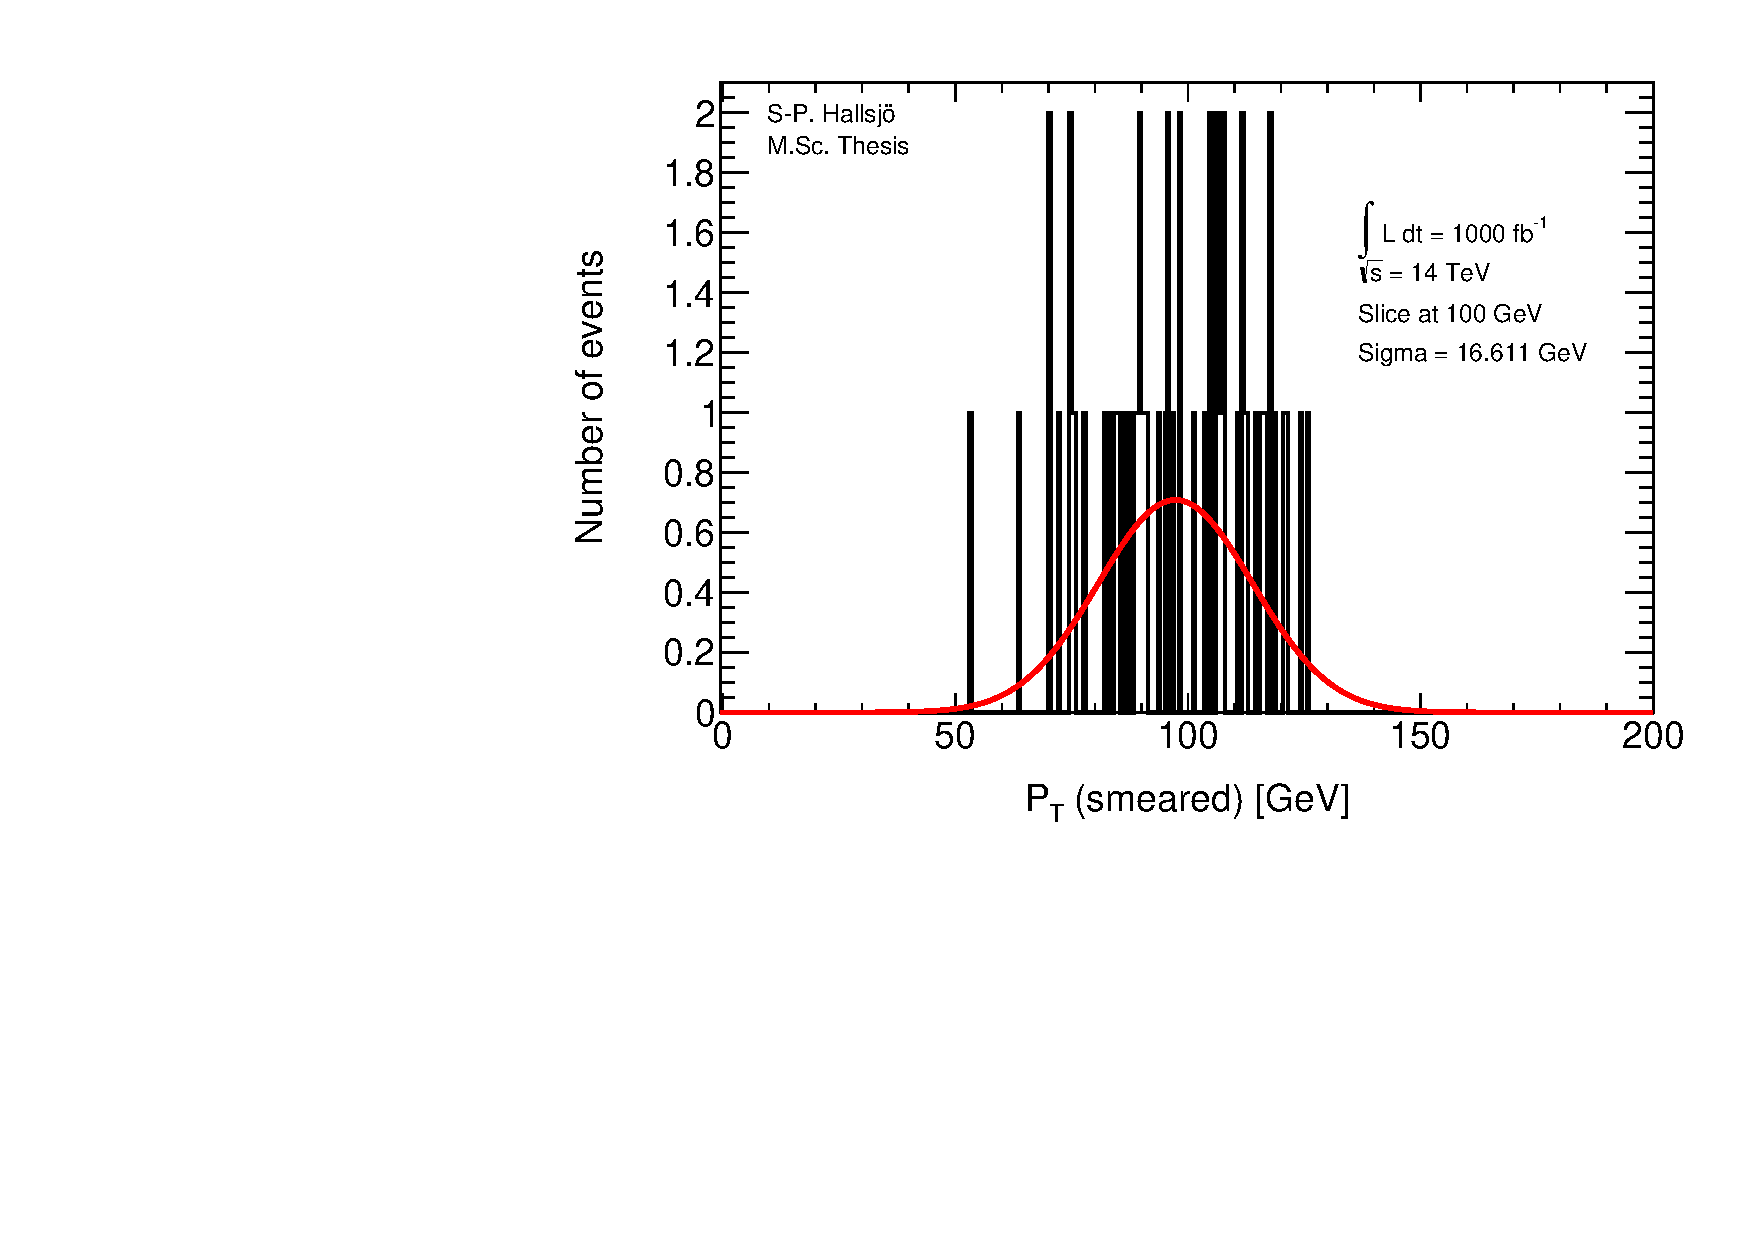
\includegraphics[width=0.5\textwidth]{jeteta4.pdf}
    }
        \hfill
\subfloat[Jet momenta after smearing \newline for $\abs{\eta}<0.8$ at $\obs{\mu}=140$. \label{fig:jet:5}]{%
      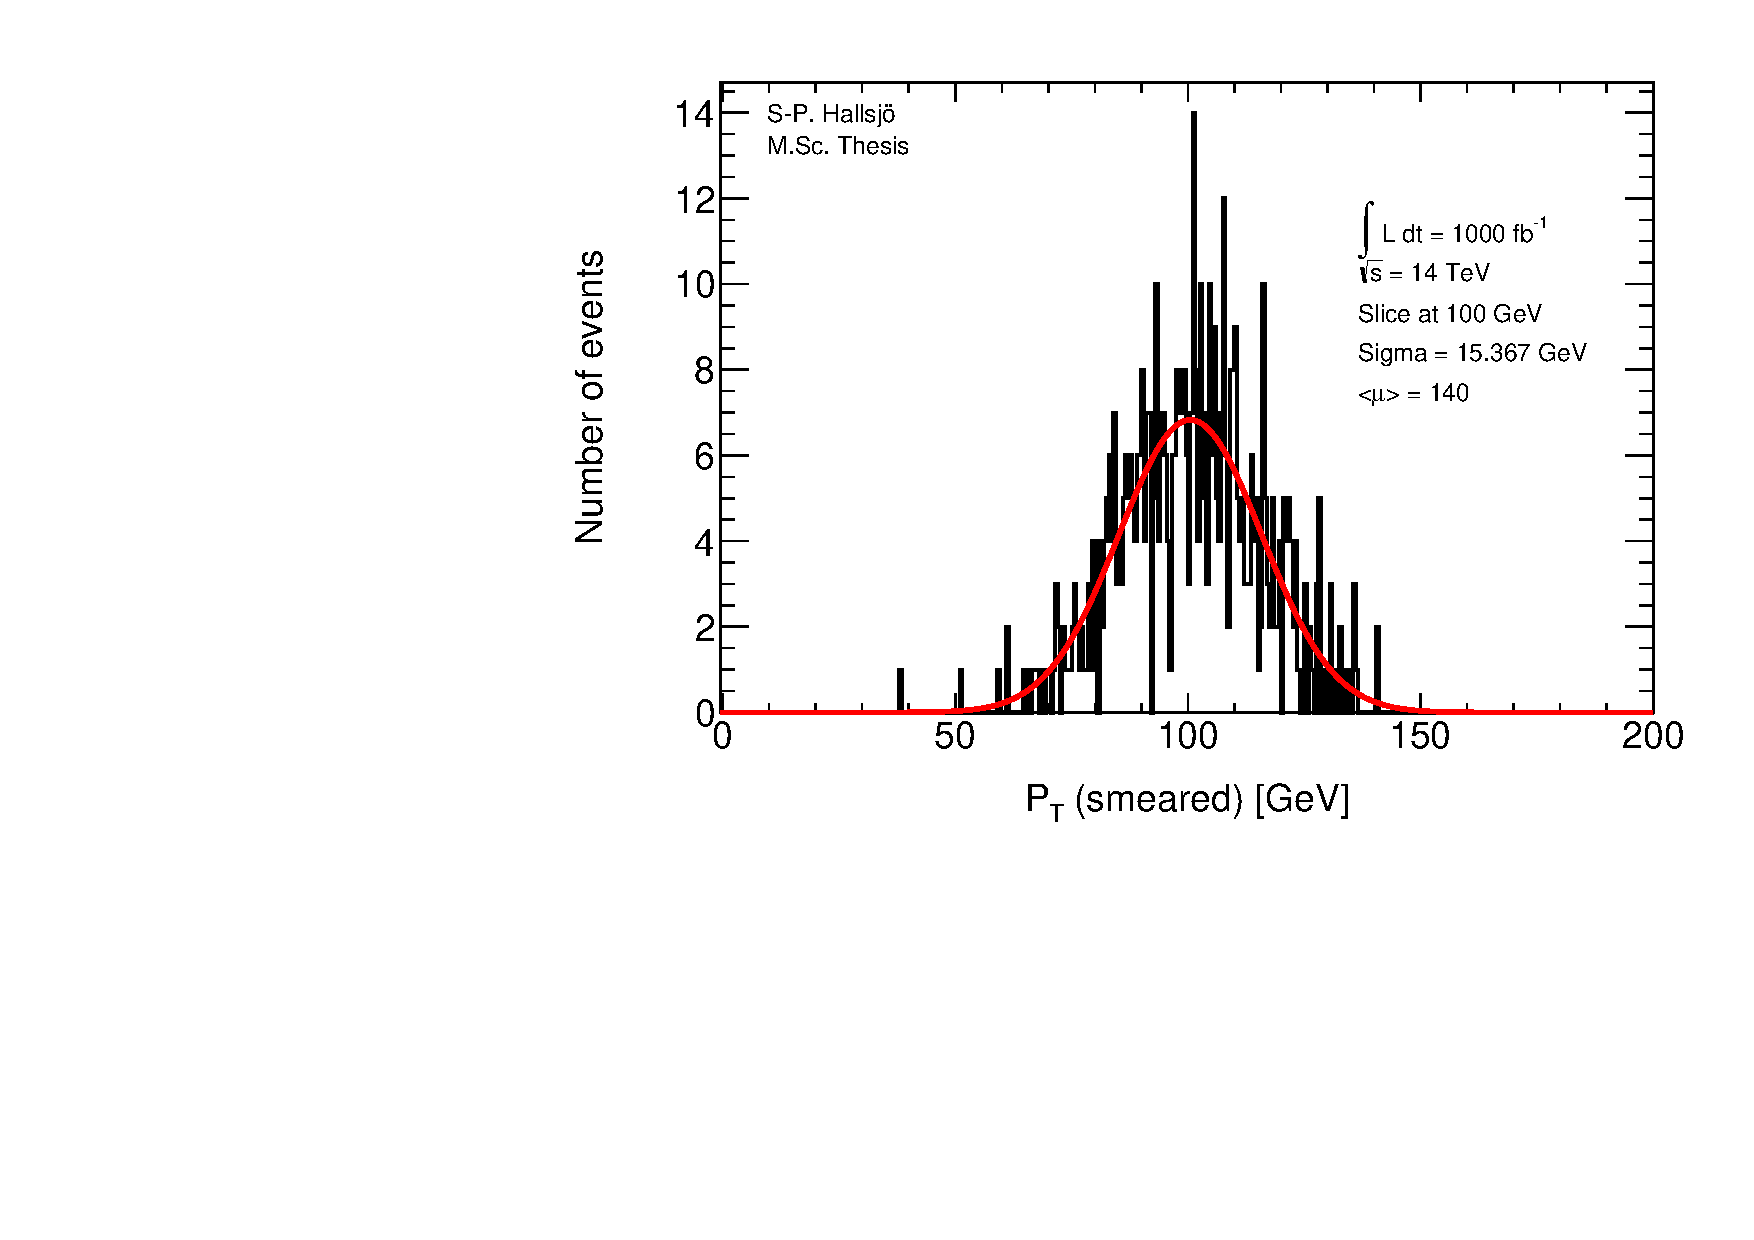
\includegraphics[width=0.5\textwidth]{jeteta1140.pdf}
    }
            \hfill
\subfloat[For $0.8<\abs{\eta}<1.2$ at $\obs{\mu}=140$. \label{fig:jet:6}]{%
      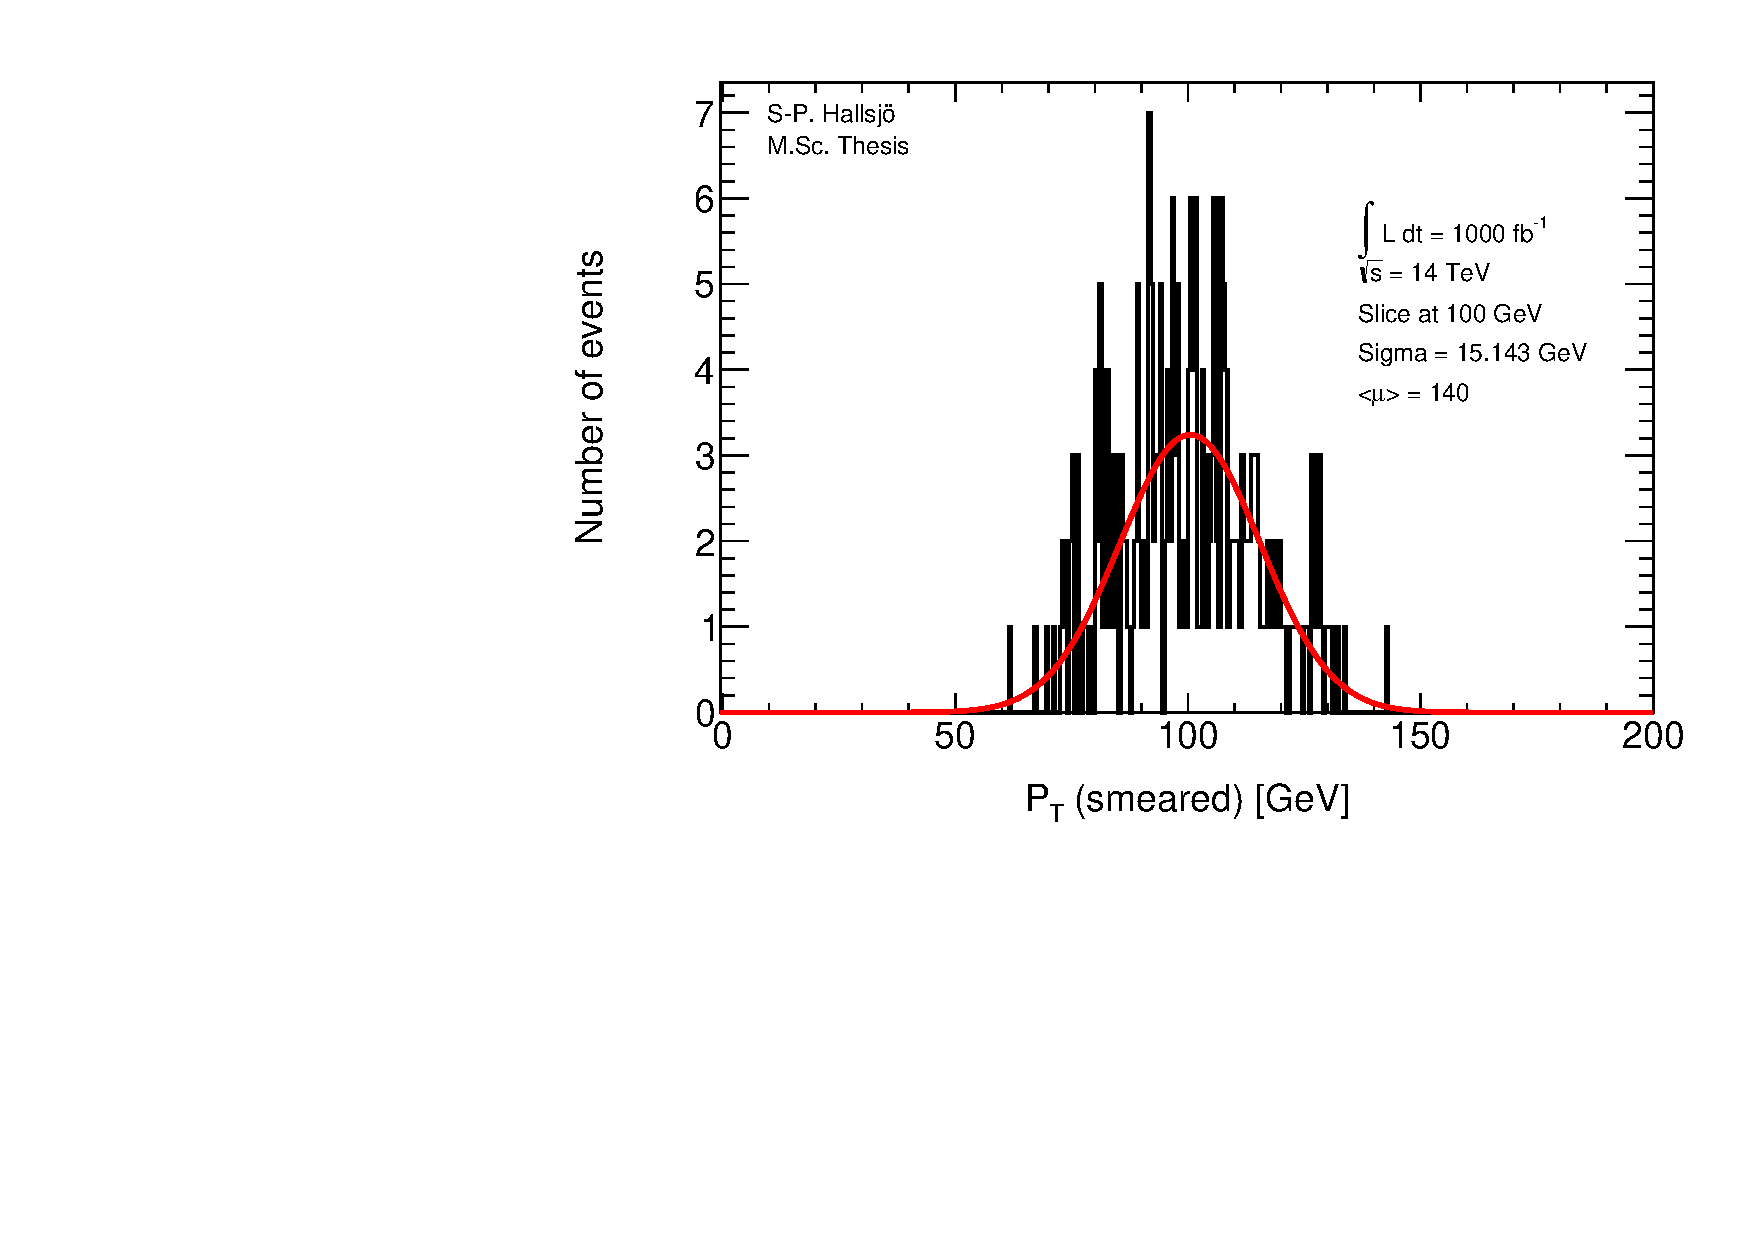
\includegraphics[width=0.5\textwidth]{jeteta2140.pdf}
    }
    \caption{Jet momenta after smearing.}
    \label{fig:jet}
\end{figure}
In \figureref{fig:jet} the Gaussian fit (red) and the data (black) are given for the jet momenta. Where $\obs{\mu}$ is the average number of simultaneous proton-proton collisions as explained in \subsectionref{sec:eo:subsec:pile}.
\subsection{Missing Transversal Energy}
The figures in this subsection are, compared to the above, given as absolute smearing. The peak value of 0 represents that the energy is unsmeared, compared to the others where the peak value represents the unsmeared energy. The unsmeared energy used here is 750 GeV.

Here the $E_T^{Miss}$ is projected down to the $x$- and $y$-axis, since these are the transverse axes, to be smeared. 
 \begin{figure}[H] %!ht
    \subfloat[$E_T^{Miss}$ smearing along the $x$-axis. \label{fig:MET:x}]{%
     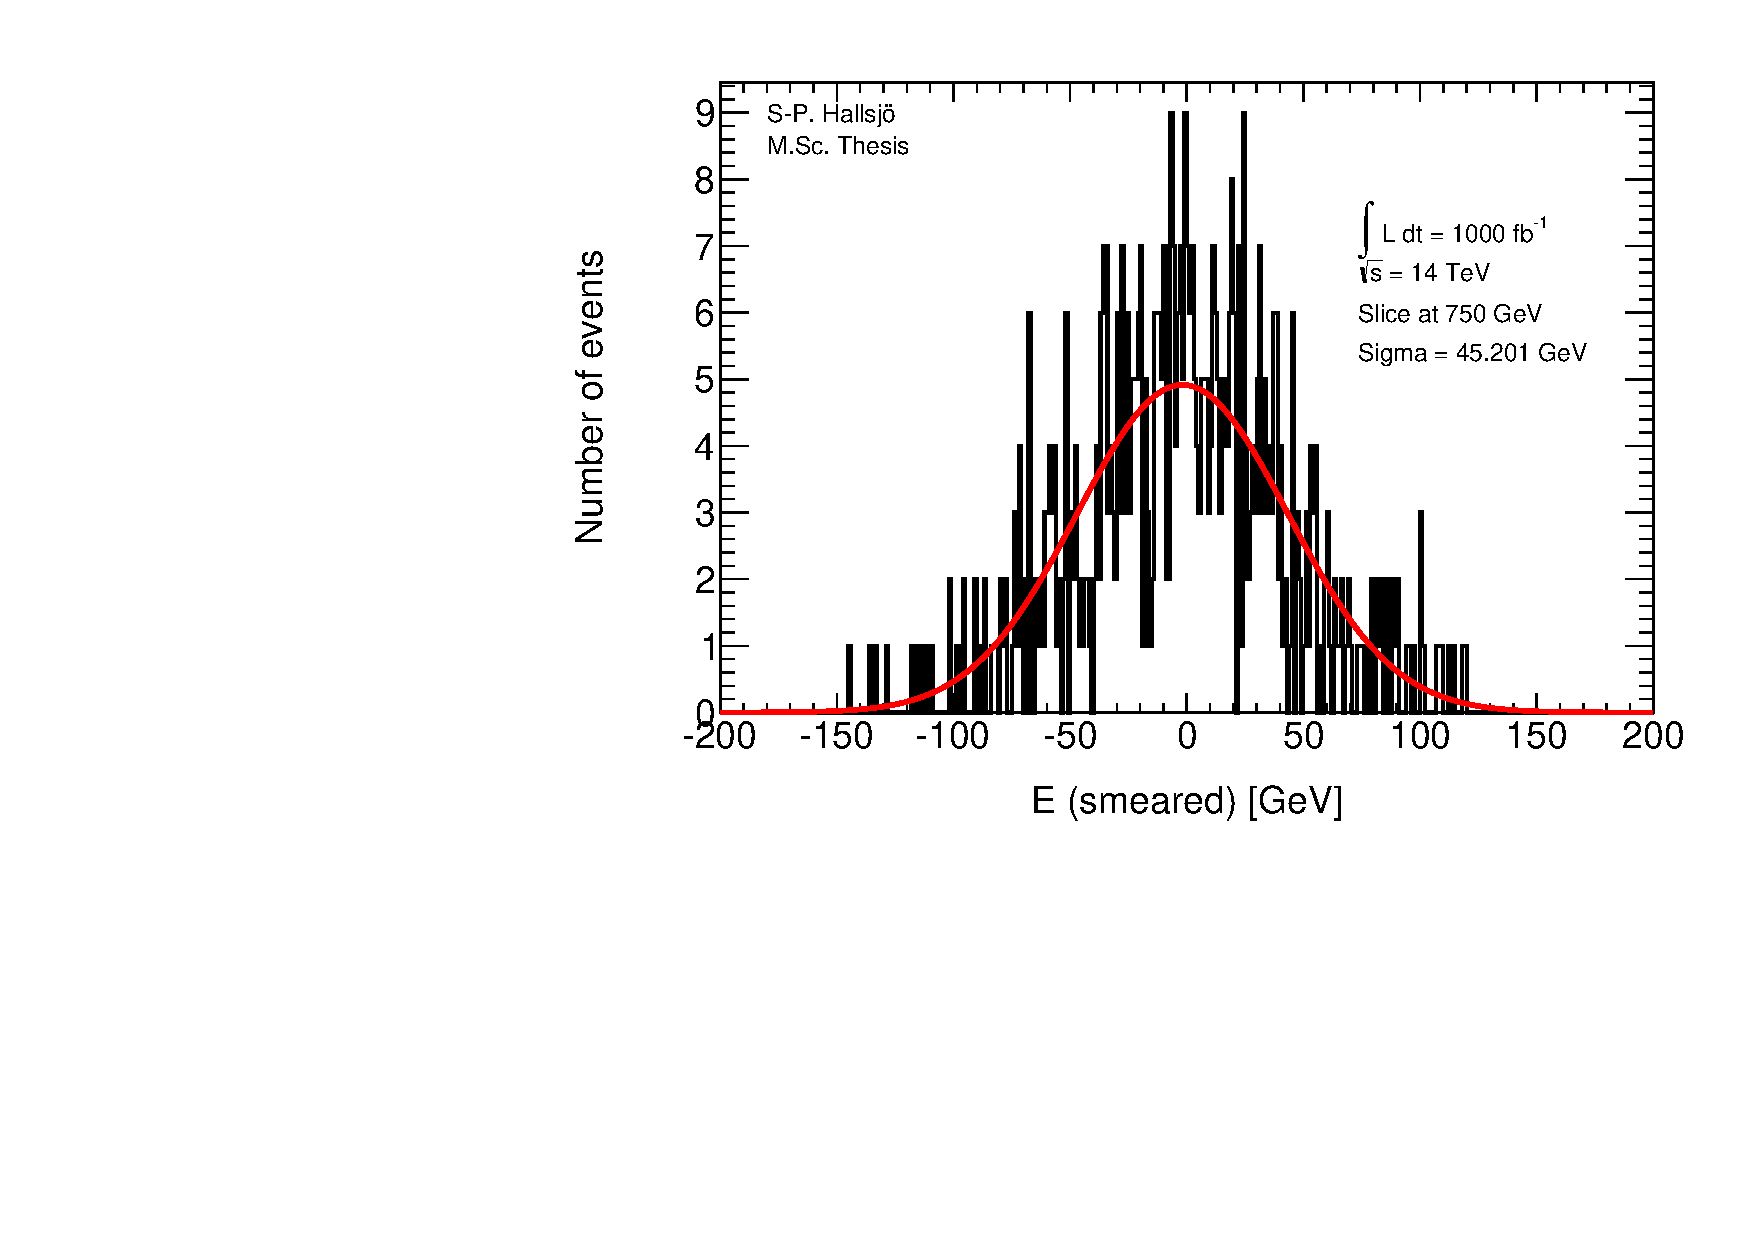
\includegraphics[width=0.5\textwidth]{METx.pdf}
    }
    \hfill
    \subfloat[$E_T^{Miss}$ smearing along the $y$-axis.\label{fig:MET:y}]{%
      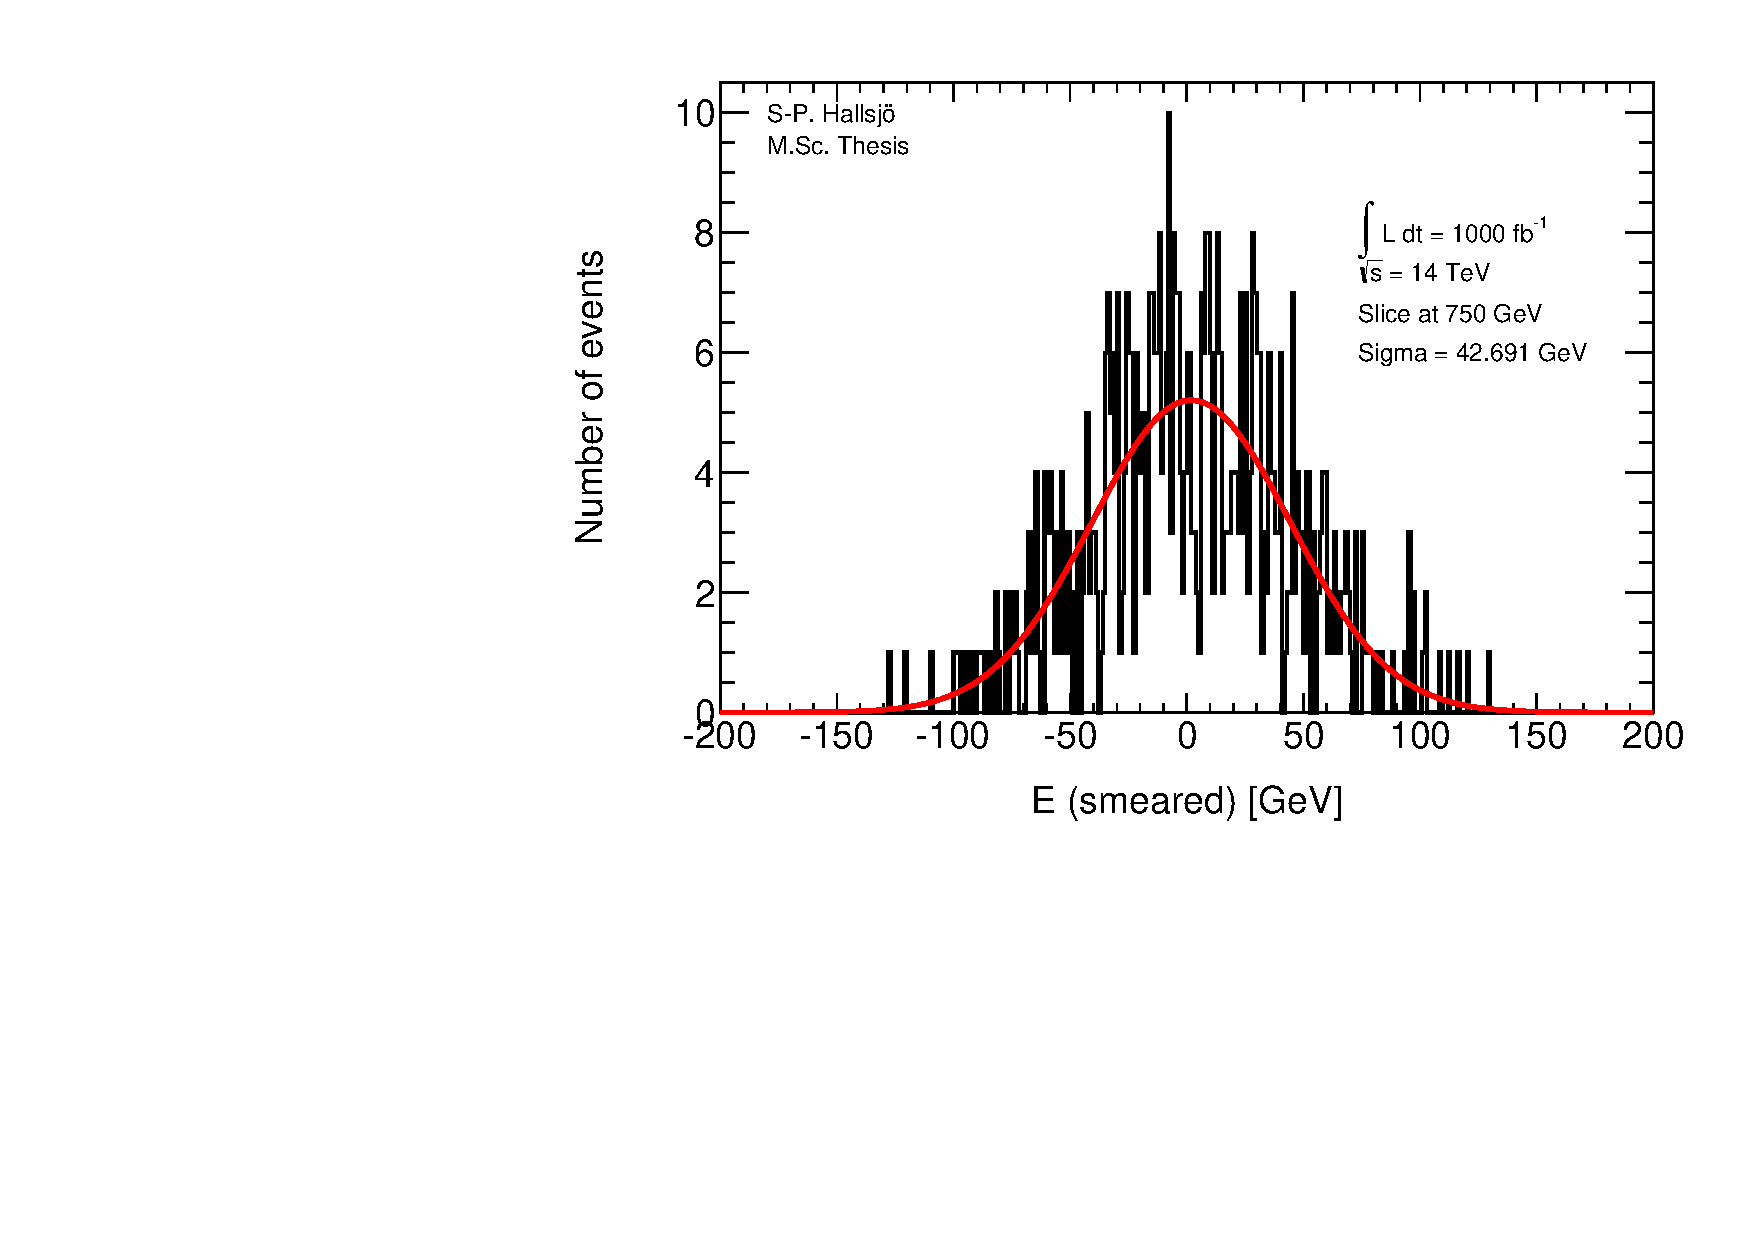
\includegraphics[width=0.5\textwidth]{METy.pdf}
    }
        \hfill
    \subfloat[$E_T^{Miss}$ smearing along the $y$-axis for $\obs{\mu}=140$.\label{fig:MET:140}]{%
      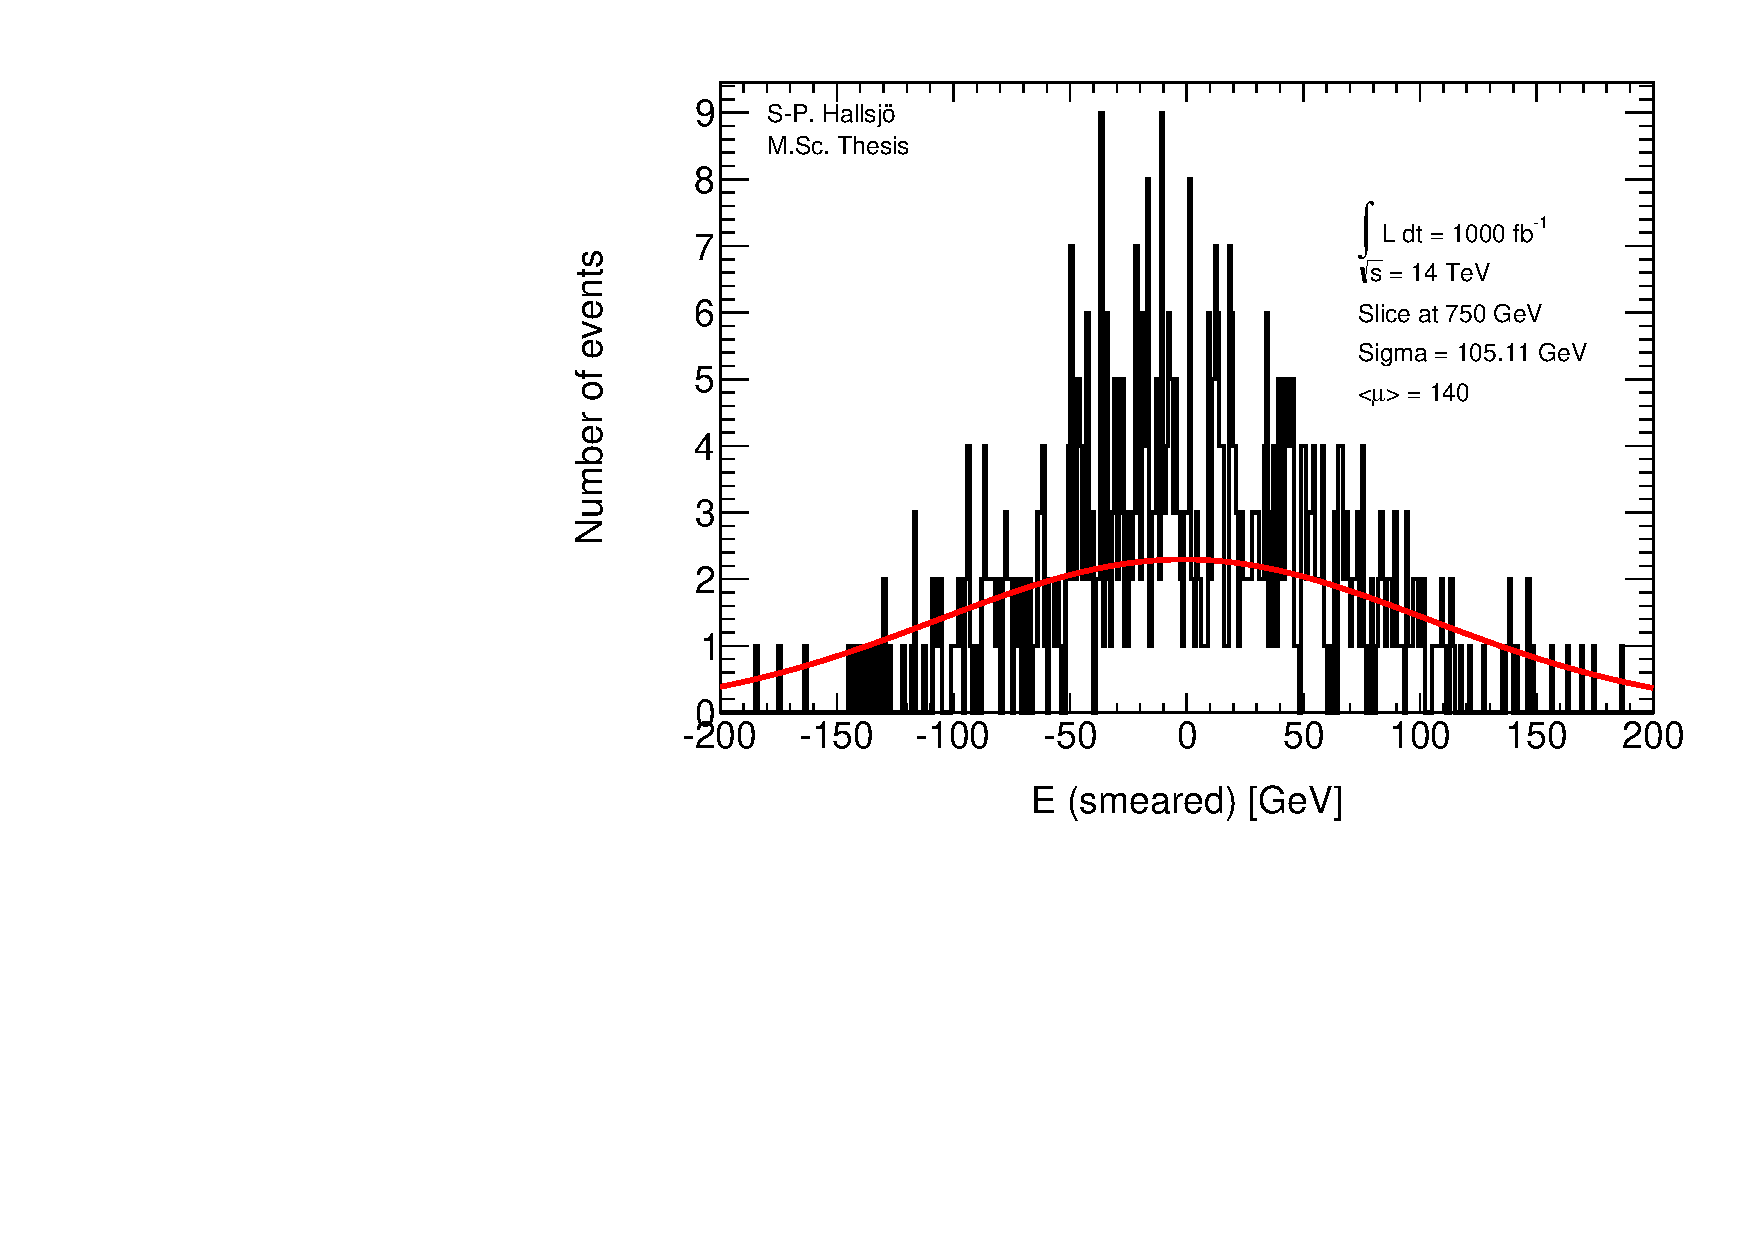
\includegraphics[width=0.5\textwidth]{mety140.pdf}
    }
   \caption{$E_T^{Miss}$ smearing plots.}
    \label{fig:MET}
  \end{figure}
\newpage
\subsection{Summary}\label{sec:res:subsec:sum}
Since the leptons and photons are all detected by fitting detector responses to different tracks, the effect of pile-up should be that there are more tracks to match, but it should not affect which ones are matched. The independence of pile-up for leptons and photons is backed up in previous research, for instance \citep{Electronperf:2011, ATLAS:LOI2}.

To validate the smearing functions, comparisons are made with \citep{ATL-PHYS-PUB-2013-004} which gave \tableref{tab:expected sigma} for the expected resolution $\sigma$.
\renewcommand{\arraystretch}{1.2} %Change back
\begin{table}[H]
\begin{center}
\begin{tabular}{|l|l|l|l|l|}
\hline
Process& $\eta$ value & Pile-up value &$\sigma$ [GeV]& Expected $\sigma$ [GeV]\\ \hline
\multirow{2}{*}{Electron}& Low $\eta$&60&$1.25 \pm 0.05$&1.18\\
&High $\eta$&60&$1.82 \pm 0.14$&1.74\\ \hline
\multirow{2}{*}{Photon} & Low $\eta$&60&$1.19 \pm 0.04$&1.18\\
&High $\eta$&60&$1.80 \pm 0.04$&1.74\\ \hline
\multirow{2}{*}{Muon} & Low $\eta$&60&$1.19 \pm 0.05$&1.50\\
&High $\eta$&60&$1.71 \pm 0.09$&2.18\\ \hline
Tau& All $\eta$&60&$10.9 \pm 0.3$&10.3\\ \hline
\multirow{6}{*}{Jet} &Low $\eta$&60&$11.4 \pm 0.4$&11.6\\
&Low $\eta$&140&$15.4 \pm 0.5$&15.8\\
&Mid low $\eta$&60&$11.5 \pm 0.5$&11.9\\
&Mid low $\eta$&140&$15.1 \pm 0.7$&15.9\\
&Mid high $\eta$&60&$11.3 \pm 0.3$&10.9\\
&High $\eta$&60&$16.6 \pm 1.5$&13.5\\ \hline
\multirow{2}{*}{$E_T^{Miss}$}&All $\eta$&60&$43 \pm 2$&48\\ 
&All $\eta$&140&$105 \pm 12$&87\\  \hline
\end{tabular}
\end{center}
\caption{Calculated $\sigma$ values compared to $\sigma$ given from the resolution given in \tableref{tab:expected sigma}. Values are given at different pile-up values for comparison.}
\label{tab:sigmaval}
\end{table}
\renewcommand{\arraystretch}{1.0} %Change back
In \tableref{tab:sigmaval} all values are given as absolute, not relative and the large difference between calculated and expected $\sigma$ for Muons and $E_T^{Miss}$ is explained by too optimistically calculated errors in $\sigma$, as discussed in \subsectionref{sec:dis:subsec:comp}.

\newpage
\section{Discussion}\label{chap:vali:sec:dis}
\subsection{Dependence of smearing on pile-up}\label{chap:vali:sec:dis:subsec:smearindep}
From the validation done it is interesting to note that the smearing functions were created from previous studies \citep{Electronperf:2011, ATLAS:LOI2} which show that detector resolution for leptons and photons is unaffected by pile-up. This may seem unexpected, however it becomes quite logical when one understands how the detectors work and the effect of pile-up.

The effect of pile-up is that extra jets are introduced to the events. These jets will not reach the muon-system and thus will not affect the identification of muons. Electron, tauons and photons are affected by it being harder to detect energy deposits in the calorimeter which are consistent with these particles, since there are more hits. However by restricting which deposits to consider it is possible to keep the resolution unaffected by pile-up. Jets and $E_T^{Miss}$ will be the most affected since they rely heavily on measurements in the calorimeter and are combined of several parts, either hadronic particles or by all the transverse missing energy. Through the formulas in \tableref{tab:expected sigma}, it is seen that the effect diminishes with an increasing energy which is consistent with the description given, and that for the high energies which are of interest in this thesis the effect of pile-up is minimal. 

\subsection{Comparison to expected results}\label{sec:dis:subsec:comp}
One of the major problems in the comparison was to get the significance of the Gaussian fit to be calculated correctly. The tool ROOT has a lot of different features which made this task somewhat difficult, specifically by calculating optimistic errors. A large contribution to the difficulty of calculating the significance lay in this being a statistical property and thus there is a statistical fluctuation in the result. 

Another problem was to retrieve the correct resolution values from Ref. \citep{ATL-PHYS-PUB-2013-004}, since it was unclear if the resolution values given were absolute or scale dependent. This has now been corrected in a new version of the paper.

\section{Conclusion}
The smearing functions work as intended within 5.8 sigma, however when using a test box and averaging the sigmas one ends up with half of this for the extreme cases, muons and $E_T^{Miss}$. This indicates that the statistical fluctuation of these values and of the error calculations are considerable. Even with this statistical fluctuation the smearing functions work as intended.